\chapter{Ausgabe} % (fold)
\label{cha:visualisierung}

In diesem Kapitel wird die konzeptuelle Ausrichtung und technische Umsetzung jenes Teils des Werkzeugs behandelt, der sich mit der Ausgabe von Information an die Benutzer beschäftigt. Im Bereich der Tangible Interface erfolgt die Ausgabe von Information zumeist kohärent mit dem Eingabemedium, eine physische Trennung zwischen Eingabe- und Ausgabekanälen wie in der herkömmlichen Mensch-Maschine-Interaktion liegt nicht vor \citep{Ullmer00}. \citet{Fishkin04} relativiert die strikte Forderung in seiner Taxonomie für Tangible Interfaces (wie in Abschnitt \ref{sub:tangibles_taxonomien} beschrieben und klassifiziert Benutzungsschnittstellen unter anderem nach dem Grad deren Ein- und Ausgabe-Kohärenz. Dementsprechend sind nicht nur jene Ausgabekanäle Gegenstand dieses Kapitels, die Information in direkter Verbindung mit den Eingabemedien zurückspiegeln, sondern auch jene, die Information auf anderen, nicht-kohärenten Wegen ausgeben.

Im ersten Abschnitt dieses Kapitels werden auf Basis der in Kapitel XY genannten Anforderung an das Werkzeug die den Benutzern mitzuteilenden Informationen identifiziert, noch ohne konkret auf die technologische Realisierung der Ausgabekanäle einzugehen. Im darauf folgenden Abschnitt die technologischen Möglichkeiten zur Ausgabe von Information betrachtet und im Anschluss hinsichtlich ihrer Eignung für die im konkreten Anwendungsfall auszugebende Information bewertet und entsprechend zugeordnet.

Im Anschluss werden auf Basis dieser grundsätzlichen Technologieentscheidung Software-Frameworks beschrieben, die die Realisierung der gewählten Ausgabekanäle ermöglichen. Die Entscheidung für ein konkretes Framework wird auf Basis der funktionalen und nicht-funktionalen Anforderungen an die Ausgabe und deren Umsetzung getroffen. Der letzte Abschnitt beschreibt die eigentliche Umsetzung der Ausgabekanäle mittels der gewählten Technologie und geht die spezifischen Eigenschaften und Implementierungsentscheidungen der vorgestellten Lösung ein.

\section{Auszugebende Information} % (fold)
\label{sec:auszugebende_information}

Den Benutzern des Systems müssen während der Modellierung unterschiedliche Information zur Verfügung gestellt werden. Einerseits ist dies Information, die das Modell selbst betrifft, andererseits muss auch Information ausgegeben werden, die Aspekte des Modellierungsablaufs beschreibt oder unterstützt.

Die das Modell betreffende Information muss folgende Aspekte abdecken:
\begin{itemize}
 \item Die Modellelemente betreffende Information (Art, Position, Benennung)
 \item Die Verbinder betreffende Information (Art, Endpunkte, Benennung)
 \item Einbettete Elemente betreffene Information (Art, Inhalt, Container)
\end{itemize}

Zur Unterstützung des Modellierungsablaufs müssen folgende Aspekte zur Verfügung gestellt werden:
\begin{itemize}
 \item Information über vergangene Modellzustände
 \item Information zur die Wiederherstellung von Modellzuständen
\end{itemize}

Hier wird bewusst noch nicht auf die technische Umsetzung dieser Ausgabe eingegangen. In den folgenden Abschnitten wird erörtert, welche grundlegenden Technologien in Frage kommen, bevor auf Basis deren Eignung und den Vorgaben aus den Technologieentscheidungen zur Informationseingabe eine konkrete Lösung ausgewählt wird.

% section auszugebende_information (end)

\section{Technologische Grundlage der Ausgabe} % (fold)
\label{sec:technologische_grundlage_der_visualisierung}

Bei der Ausgabe von Information muss im Falle von Tangible Interfaces zwischen Ansätzen mit unterschiedlich stark ausgeprägter Kohärenz mit den Eingabekanälen unterschieden werden. Unter Kohärenz ist hier zu verstehen, das jene Artefakte, die zur Eingabe verwendet werden gleichzeitig auch die Reaktion des Systems -- also die Ausgabe -- wiederspiegeln. In der von \citet{Fishkin04} vorgeschlagenen Taxonomie (siehe Abschnitt XY) werden in der Dimension „Embodiment“ auch Werkzeuge als Tangible Interfaces klassifiziert, bei denen die Ausgabe vollständig von der Eingabe entkoppelt ist. Diesem Verständnis folgt auch diese Arbeit.

Bei Tabletop Interfaces bietet sich die Tischoberfläche als Ausgabemedium an, um kohärente Informationsausgabe zu gewährleisten. Die Tischoberfläche dient hier wie in Kapitel \ref{cha:input_&_interpretation} beschrieben der Eingabe und kann durch unterschiedliche technologische Maßnahme auch zur Ausgabe genutzt werden. Eine weitere Möglichkeit, die Ausgabekohärenz bei Tabletop Interfaces sicherzustellen bzw. zu steigern, ist die Verwendung der zur Interaktion mit dem System verwendeten Tokens als Ausgabemedium. Je nach verfolgtem Ansatz (bzw. einer Kombination) sind unterschiedliche technische Maßnahmen zu setzen. In den folgenden Abschnitten werden die hier erwähnten grundsätzlich in Frage kommenden Ansätze betrachtet und im Anschluss hinsichtlich ihrer Eignung für das hier entwickelte System beurteilt. Basierend auf der grundsätzlichen Technologieentscheidung werden im Anschluss unterschiedliche technische Lösungen zur Erfüllung der Anforderungen beschrieben.

\subsection{Ansätze zur kohärenten Ausgabe} % (fold)
\label{sub:kohärente_ausgabe}

In diesem Abschnitt werden Ausgabeansätze behandelt, die nach \citep{Fishkin04} in der Embodiment-Dimension den Ausprägungen „full“ oder „nearby“ zuzuordnen sind. Die Ausgabe erfolgt bei den hier vorgestellten Ansätzen also direkt über die Eingabetokens („full“) oder ist räumlich unmittelbar in der Umgebung der Tokens angesiedelt.

\subsubsection{Darstellung auf der Tischoberfläche} % (fold)
\label{ssub:darstellung_auf_der_tischoberfläche}

Bei Tabletop-Interfaces ist die Nutzung der Tischoberfläche ein naheliegender und gängiger Ansatz zur Realisierung der Ausgabekanäle. Die Ausgabe erfolgt hierbei visuell, also durch die Darstellung der auszugebenden Information. Ein derartig ausgestaltetes Interface ist hinsichtlich seiner Ausprägung in der Embodiment-Dimension als „nearby“ zu klassifizieren. Technologisch kommen zur Darstellung horizontal eingesetzte Bildschirme oder Oberflächen, auf die projiziert werden kann, in Frage.

Bei der Verwendung von Bildschirmen sind die Größe der zur Anzeige verwendbaren Oberfläche sowie die zur Anzeige verfügbare Auflösung (also indirekt die Größe eines Bildpunktes) wesentliche Kriterien. Bei heute verfügbaren \gls{LCD}-Modulen mit Größen bis zu 132 cm in der Diagonale und Auflösungen von 1920 x 1080 Bildpunkten ist die Technologie soweit ausgereift und verfügbar, das dieser Ansatz grundsätzlich für den Einsatz in Tabletop Interfaces in Frage kommt. Vorteile sind die geringe Bauhöhe der Ausgabeeinheit (im Vergleich zu den im Folgenden vorgestellten Projektions-Lösungen). Nachteile sind die relative geringe Leuchtstärke, die einen Einsatz bei Tageslichtbedingungen schwierig machen sowie die Blickwinkelabhängigkeit, die bei horizontalem Einbau der Anzeigeeinheit stärker zum Tragen kommt als bei herkömmlicher vertikaler Verwendung.

Als Alternative zur Verwendung von aktiven Anzeigeeinheiten können Projektoren verwendet werden, die die darzustellende Information auf die Tischoberfläche projizieren. Hier ist zwischen Lösungen zu unterscheiden, bei denen die Projektion von oben erfolgt und jenen, die von unten auf eine durchscheinende Tischoberfläche projizieren. Bei ersteren muss der Projektor in ausreichender Höhe über der Tischoberfläche angebracht werden, um das projizierte Bild die notwendige Fläche abdecken zu lassen. Bei beschränkter Höhe nach oben kann ein Projektor mit Weitwinkelobjektiv oder ein Umlenkspiegel benutzt werden, der durch eine Vergrößerung des Abstands zwischen Projektor und Oberfläche auf einer nicht vertikalen Achse die notwendige Bauhöhe reduziert. Der größte Nachteil dieser Lösung ist die Abschattung der projizierten Information bei Manpulationen der Tokens auf der Oberfläche. Um dies zu vermeiden kann auch von unten auf eine durchscheinende Oberfläche projiziert werden. Bei diesem Lösungsansatz kommt es zu keinerlei Abschattungen, die Information wird wie bei Einsatz eines Bildschirms ständig angezeigt. Nachteilig wirkt sich hier der durch den Einsatz einer durchscheinenden Oberfläche verursachte Leuchtkraftverlust aus. Bei dieser Form der Projektion wird immer ein Teil des durch den Projektor ausgestrahlten Lichts von der Oberfläche nach unten zurück reflektiert. Im Gegensatz zur Projektion von oben ist dadurch der Kontrast der Darstellung wesentlich geringer. Für den Einsatz unter Tageslichtbedingungen erscheint also der erstgenannte Ansatz generell besser geeignet. Kritischer ist bei der Projektion von unten der notwendige Abstand zwischen Projektor und Tisch, da sich dieser direkt auf die Höhe des Tisches auswirkt. Um eine akzeptable Bauhöhe zu erreichen -- also den Tisch durch durchschnittliche große Personen bedienbar zu halten (Höhe nicht mehr als etwa 100 cm) -- ist hier der Einsatz eines Umlenkspiegels nahezu unabdingbar. Beiden Projektions-Ansätzen gleich ist, dass die abzudeckende Oberfläche variabel durch den Abstand des Projektors gewählt werden kann. Grenzen sind hier nach unten die Fokussierbarkeit des Projektors bei kleinen Abständen und nach oben die Abnahme der Projektionshelligkeit bei großen Abständen. Bei großen Oberflächen ist zudem auf die verfügbare Auflösung des Projektors zu achten, da die Größe eines Bildpunktes mit zunehmendem Abstand so ansteigt, dass eine feinauflösende Projektion der Information auf der Oberfläche nicht mehr möglich ist.

% subsubsection darstellung_auf_der_tischoberfläche (end)

\subsubsection{Aktive Anzeige auf Tokens} % (fold)
\label{ssub:aktive_anzeige_auf_tokens}

Alternativ zur Darstellung auf der Tischoberfläche können bei Tabletop-Interfaces auch die Tokens selbst als Ausgabekanal dienen. Die hier das Eingabemedium gleich dem Ausgabemedium ist, ist diese Form der Ausgabe hinsichlich der Embodiment-Dimension in die Ausprägung „full“ einzuordnen. Technologisch können je nach Art der darzustellenden Information Tokens mit Displays ausgestattet werden oder lediglich visuelle Statusanzeigen beinhalten, die Feedback über den aktuellen Zustand des Tokens geben. In beiden Fällen müssen die Tokens generell mit Elektronik und Energieversorgung ausgestattet sein und die Möglichkeit haben, selbst oder über eine Verbindung mit der Infrastruktur ihren Zustand festzustellen.

Um textuelle oder grafische Information auf Tokens darzustellen ist die Verwendung von Displays notwendig. Bei der Verwendung von herkömmlichen \gls{LCD}-Displays ist durch die notwendige Hintergrundbeleuchtung sowie der notwendigen Stromversorgung zur Aufrechterhaltung der Anzeige der Energieverbrauch verhältnismäßig hoch. Alternativ können neuere Technologien wie \gls{OLED}- (REF) oder eInk-Displays (REF) verwendet werden. \gls{OLED}s bestehen aus organischen Materialien und benötigen keine Hintergrundbeleuchtung, das das Material selbst Licht emmitiert. eInk verwendet eine papierartige Oberfläche zur Anzeige, strahlt selbst kein Licht aus und ist deshalb auf Umgebungshelligkeit zur Verwendung angewiesen. eInk bietet in hellen Umgebungen die besten Kontrastverhältnisse (vergleichbar mit bedrucktem Papier) kann allerdings beim heutigen Stand der Entwickung keine Farben darstellen. Der größte Vorteil von eInk liegt in der Eigenschaft, dass die Anzeige auch ohne Energieversorgung aufrecht bleibt -- Energie ist lediglich zur Änderung des Display-Inhalts notwendig.

Durch das Wegfallen der Hintergrundbeleuchtung sind \gls{OLED}- und eInk-Displays wesentlich dünner als \gls{LCD}-Module und können auch auf nicht ebenen Oberflächen angebracht werden. Allen drei Ansätzen gleich ist, dass zur Ansteuerung des Anzeigemoduls Elektronik notwendig ist, die die darzustellende Information auf die zur Verfügung stehen Bildpunkte abbildet und das Display entsprechend ansteuert.

Neben der Verwendung eines Displays kann der Status eines Tokens auch mit Leuchtanzeigen in der Form von \glspl{LED} visualisiert werden. Der Nachteil dieses Ansatzes ist die schwierige Realisierbarkeit von komplexen Statusanzeigen - durch die auf zwei Zustände (ein/aus) beschränkte Aussagekraft einer \gls{LED} sind andere als bipolare Visualisierungen schwer zu realisieren. Möglich ist die Verwendung von mehreren \glspl{LED}, wobei diese rasch schwer erfassbar wird, wenn dadurch mehrere voneinander unabhängige Aussagen visualisiert werden. Lediglich die Kopplung mehrere \glspl{LED} zur aussagekräftigen Visualisierung von dynamischen Zuständen hat sich als intuitiv erfassbar und verständlich erwiesen (REF Zuckerman Flow Blocks). So können gekopplte \glspl{LED} z.B. dazu verwendet werden, Flussrichtungen von Ressourcenströmen anzuzeigen, indem eine \gls{LED}-Reihe entweder von links nach rechts oder von rechts nach links angesteuert wird. Auch beim Einsatz von \glspl{LED} ist einer ständige Energieversorgung notwendig. Zur Reduktion des Energieverbrauchs können wiederum die oben genannten Alternativ-Technologien \gls{OLED} und eInk zum Einsatz kommen, wobei diese aktuell nicht in den Bauformen herkömmlicher \glspl{LED} angeboten werden. eInk-Anzeigen eignen sich aufgrund ihrer langsamen Schaltdauer außerdem nicht für die Realisierung dynamischer Anzeigen.

% subsubsection aktive_anzeige_auf_tokens (end)

\subsubsection{Token mit Aktuatoren} % (fold)
\label{ssub:tokens_mit_aktuatoren}

Neben der Verwendung von Displays zur Realisierung eines „full embodied“ Ausgabekanals können Tokens auch mit Aktuatoren ausgestattet werden, die es erlauben, das Token bzw. dessen Verhalten selbst ohne direkte Benutzerinteraktion zu beeinflussen. Beispiele für Aktuatoren sind unter anderem Vibrationsmodule oder mechanische Einheiten zur Veränderung der äußeren Form des Tokens oder dessen Position (auf der Tischoberfläche). Der Einsatz von Aktuatoren ist ob der technologischen und anwendungsspezifischen Vielfalt nicht generisch beschreibbar wie das bei reinen optischen Anzeigeeinheiten der Fall war. Aktuatoren müssen auf den jeweiligen Anwendungsfall abgestimmt sein. Ihr Einsatz ist im Allgemeinen eher disruptiv, unterbricht durch die vom Benutzer nicht selbst ausgelöste Interaktion dessen aktuelle Aktivität und zieht die Aufmerksamkeit auf sich. Dies kann im einzelnen Anwendungsfall erwünscht sein, kann aber zu unerwünschten Effekten bei der Verwendbarkeit des Systems führen.

Wie bei Anzeigemodulen müssen auch hier die Tokens mit Energieversorgung ausgestattet sein und mit Elektronik integriert werden, die für die Ansteuerung der Aktuatoren sorgt.

Im Bereich der Tabletop Interfaces ist die Verwendung von Aktuatoren eher selten anzutreffen. Im Bereich der Ambient Interfaces kann der Einsatz von Aktuatoren aber sinnvoll sein, wenn sich das Interface so in die Umgebung seines Einsatzbereichs integrieren kann (REF Bsp ... Ferscha Blubbersäule?).

% subsubsection tokens_mit_aktuatoren (end)
% subsection kohärente_ausgabe (end)

\subsection{Ansätze zur entkoppelten Ausgabe} % (fold)
\label{sub:entkoppelte_ausgabe}

Ansätze zur enkoppelten Ausgabe sind solche, die von \citet{Fishkin04} in seiner Taxonomie in der Embodiment-Dimension unter den Ausprägungen „environment“ oder „distant“ eingeordnet werden. 

„Environmental Embodiment“ ist dann gegeben, wenn Eingabe- und Ausgabekanäle räumlich nicht kohärent sind, aber Eingaben trotzdem offensichtlich Reaktionen in der unmittelbaren Umgebung auslösen. Klassische von Fishkin genannte Ansätze sind hier Audiokanäle aber auch die Veränderung von Umgebungslicht oder Temperatur. Auch olfaktorische Interfaces wären in diese Kategorie einzuordnen. In den folgenden Abschnitten werden jedoch ausschließlich audio-basierte Kanäle beschrieben, da diese im Bereich der Tabletop Interfaces Relevanz besitzen (etwa in REF reacTable und REF TEI Paper von Däne)

Die Ausprägung „distant“ kennzeichnet Ansätze, in denen die Eingabekanäle räumlich von den Ausgabekanälen vollkommen enkoppelt sind bzw. entkoppelt werden können. Ein Kriterium zur Einordung eines Ansatzes unter „distant“ ist, dass Benutzer zur Beobachtung der Ausgabe nicht mehr die Eingabe im Blickfeld haben können (was bei allen anderen Ausprägungen möglich ist). Klassische Vertreter dieses Ansatzes sind alle Ansätze die auf der Darstellung von Information auf herkömmlichen Bildschirmen oder Projektionsflächen basieren.

\subsubsection{Darstellung auf Monitoren} % (fold)
\label{ssub:monitore}

Bei der Darstellung von Information auf Bildschirmen kommen die auch in der herkömmlichen Desktop-basierten Mensch-Maschine-Interaktion gängigen Anzeigetechnologien zur Anwendung. Im Kontext von Tabletop Interfaces ist bei Monitoren auf die Sichtbarkeit der Information für alle an der Interaktion beteiligten Personen zu achten -- diese ist nicht nur von der Entfernung zum Monitor abhängig sondern bei den heute gängigen \gls{LCD}-Displays auch vom Blickwinkel. Gegebenenfalls müssen mehrere Monitore verwendet werden, auf denen entweder simultan die gleiche  Information dargestellt wird oder -- abhängig von der Anwendung -- lediglich für die jeweils eingenommene Perspektive relevante Information angezeigt wird. Mit Monitoren kann auch eine vollständig räumlich entkoppelte Darstellung realisiert werden, indem die darzustellende Information auf entfernte Displays übertragen wird. So kann zum Beispiel die Interaktion auf einem Tabletop Interface bzw. deren Auswirkungen auch räumlich entfernt verfolgt werden.

Generell muss bei entkoppelten Ausgabekanälen darauf geachtet werden, dass bei Interaktionen mit den tangiblen Eingabekanälen entsprechend eindeutig zuzuordnendes Feedback über die Ausgabekanäle rückgespiegelt wird. Bei Tabletop Interfaces ist hierbei (wiederum abgängig von der Anwendung) eine schematische Darstellung der Tischoberfläche mit einer Kenntlichmachung des Bereichs, in dem eine Interaktion erkannt wurde, sinnvoll.

% subsubsection tokens_mit_aktuatoren (end)

\subsubsection{Projektion auf entfernte Oberflächen} % (fold)
\label{ssub:projektion}

Bei Ausgabe mittels Projektion auf entfernte Oberfläche (im Sinne von Oberflächen, die nicht dem eigentlichen Interface zuzuordnen sind) sind Aspekte wie Größe des Bildes oder Blickwinkelabhängigkeit der Darstellung meist keine Herausforderung. Mit einem Projektor können zumeist alle Benutzer ausreichend mit Information bedient werden. Ansonsten gelten die obigen Ausführungen hinsichtlich eindeutig zuzuordnendem Feedbacks analog.

Bei individueller Nutzung eines Tangible Interfaces ist in der Verwendung von Bildschirm oder Projektor noch ein unterschiedlich hoher Grad an Privatheit der Ausgabekanäle festzustellen. Während Bildschirme eher dem mit dem System interagierenden Individuum als Ausgabekanal vorbehalten bleiben, sind projezierte Informationen quasi öffentlich verfügbar. Abhängig vom Anwendungsszenario des Tangible Interfaces kann dies erwünscht sein oder nicht.

% subsubsection tokens_mit_aktuatoren (end)

\subsubsection{Audio-basierte Ausgabekanäle} % (fold)
\label{ssub:audioausgabe}

Audio-basierte Ansätze werden hier als Vertreter von Ausgabekanälen vorgestellt, die in die Kategorie „environmental Embodiment“ eingeordnet werden. Audio-Interfaces arbeiten mit akustischer Ausgabe von Information, die im Allgemeinen in Zusammenhang mit den Eingaben am Tangible Interface stehen. 

Die ausgegebene Information kann abstrakt, codiert oder natürlichsprachlich sein. Unter „abstrakter“ Information werden hier akustische Ausgaben verstanden, die nicht unmittelbar Bedeutung im sprachlichen Sinn tragen sondern auf Meldodien oder anderen Klangmustern basieren. Derartige Formen der Ausgabe kommen vor allem im künstlerischen Bereich zu Einsatz (REF reactable, TEI-Däne). „Codierte“ akustische Ausgabe deckt alle Bereiche ab, in denen Klänge verwendet werden, um Information zu transportieren, ohne das diese selbst in diesen Klängen abgebildet ist. Beispiele hierfür sind Signaltöne, die einen Fehler melden oder anderweitig die Aufmerksamkeit der Benutzer auf sich ziehen sollen. Unter „natürlichsprachlicher“ akustischer Ausgabe werden hier schließlich alle Ansätze eingeordnet, die die Ausgabe der Information direkt in Sprache umgesetzt vornehmen. Dies kann mittels gespeicherten (Teil-)Ansagen oder mittels Sprachsynthese realisiert werden. Im Gegensatz zu den anderen beiden Formen der akustischen Ausgabe ist die natürlichsprachliche Ausgabe abhängig vom Sprachverständnis der Benutzer und deshalb in einer bestimmten Konfiguration nur für einen beschränkten Benutzerkreis nutzbar.

Akustische Ausgabe ist allen ihren Ausprägungen der Embodiment-Dimension „environment“ zuzuordnen. Sie kann im Allegemeinen (ohne den Einsatz von Ohrhörern) von allen sich im Umfeld des Interfaces befindlichen Personen wahrgenommen werden. Bei codierter Ausgabe muss darauf geachtet werden, das die Interpretation der Signale bekannt ist bzw. durch unterstützende (visuelle oder taktile) Maßnahmen erschließbar wird.

% subsubsection tokens_mit_aktuatoren (end)

% subsection entkoppelte_ausgabe (end)

\subsection{Technologie-Entscheidung} % (fold)
\label{sub:output_ansatz_entscheidung}

Auf Basis der in Abschnitt \ref{sec:auszugebende_information} festgelegten auszugebenden Information und den im letzten Abschnitt beschriebenen technologischen Alternativen zur Realisierung unterschiedlich ausgeprägter Ausgabekanäle können nun grundsätzliche Technologieentscheidungen getroffen werden.

Für die im Kontext der eigentlichen Modellierung auszugebenden Information (Benennungen, \ldots) erscheint ein kohärenter Ansatz am geeignetsten, da die Information inhärenter Bestandteil des Modells ist und deshalb räumlich mit den physischen Elementteilen (den Tokens) in eine einheitliche Modellsicht integriert werden sollte. Mit der bereits in Kapitel \ref{cha:input_&_interpretation} aurgumentierten Entscheidung für passive Tokens ist die Projektion der Information auf die Tischoberfläche der einzig naheliegende Ansatz. Dabei wird im Sinne der kompakteren Bauweise und der nicht vorhandenene Einschränkung bezüglich Verdeckungen der Projektion durch modellierende Personen ein Lösungsansatz mit Projektion auf die Unterseite bevorzugt. Die kompaktere Bauweise ergibt sich aus der Tatsache, dass der Innenraum des Tisches ohnehin bereits für die Erfassung der Tokens durch die Kamera genutzt wird und dass bei gleichzeitiger Nutzung für die Projektion ein Auf- bzw. Überbau des Tisches zur Aufnahme des Projektors entfällt.

Die Ausgabe vergangener Modellzustände erscheint mit den gegebenen technologischen Rahmenbedingungen hingegen nicht für kohärente Ausgabe geeignet. Passive Tokens können ihre Position nicht selbständig verändern, weshalb die auf der Tischoberfläche vorhandenen Modellierungstokens immer an den Positionen liegen, an denen sie sich im aktuelleń Modellzustand befinden. Eine kohärente Ausgabe von vergangenen Modellzuständen auf der gleichen Oberfläche ist deswegen nicht möglich -- es käme zu Überdeckungen der physischen und projizierten Modelldarstellungen. Aus diesem Grund wird Zweck ein zweiter Ausgabekanal verwendet, der diese Modellierungshistorie nicht kohärent darstellt. Akustische Ansätze erscheinen ob der Komplexität der Modelle und deren inhärent visuell-diagrammatischen Darstellung im Gegensatz zu visuellen Ansätzen als ungeeignet. Zu diesem Zweck wird also ein Bildschirm- oder Projektions-basierter Ausgabekanal implementiert. Dies hat auch den Vorteil, dass ins Modell zu integrierende digitale Ressourcen in ihrer „natürlichen“ Umgebung, dem Bildschirm eines Rechners manipuliert und ausgewählt werden können. Letzendlich lässt sich ein derartiger Ausgabekanal beliebig replizieren und auch für entfernte Ausgabe des Modellzustandes nutzen.

Konkret werden für das vorgestellte System also zwei Ausgabekanäle genutzt, die beide auf der visuellen Darstellung von Information basieren und sich in ihrer Ausprägung der „Embodiment“-Dimension nach \citep{Fishkin04} unterschieden. Der hauptsächliche Ausgabekanal ist die Tischoberfläche, auf ihr wird Information „nearby“ ausgegeben. Für Funktionen, für die diese kohärente Ausgabeform nicht adäquat einsetzbar ist, existiert ein zweiter, „distant“ Ausgabekanal in Form eines Bildschirms oder eines externen Projektors. Dieser Kanal kann in zwei Modi betrieben werden. Wird er nicht benötigt, kann er entweder deaktiviert werden (und so den Fokus auf den primären Ausgabekanal, die Tischoberfläche, lenken) oder synchron mit der Tischoberfläche den aktuellen Modellzustand anzeigen. Zweiteres ist sinnvoll, wenn der Modellierungsprozess auch von Personen verfolgt werden können soll, die sich nicht unmittelbar bei der Modellieruungsoberfläche befinden. 

Hardwareseitig ergibt sich aus dieser Entscheidung der in Abbildung \ref{fig:img_ImplementierungInput_TischSeitenansichtOutput} dargestellte Aufbau. Dabei kann der in der Standardkonfiguration vorhandene Bildschirm als Ausgabekanal je nach den räumlichen Gegebenheiten und dem konkreten Anwendungsszenario durch einen Projektor ersetzt werden.

\begin{figure}[htbp]
	\centering
		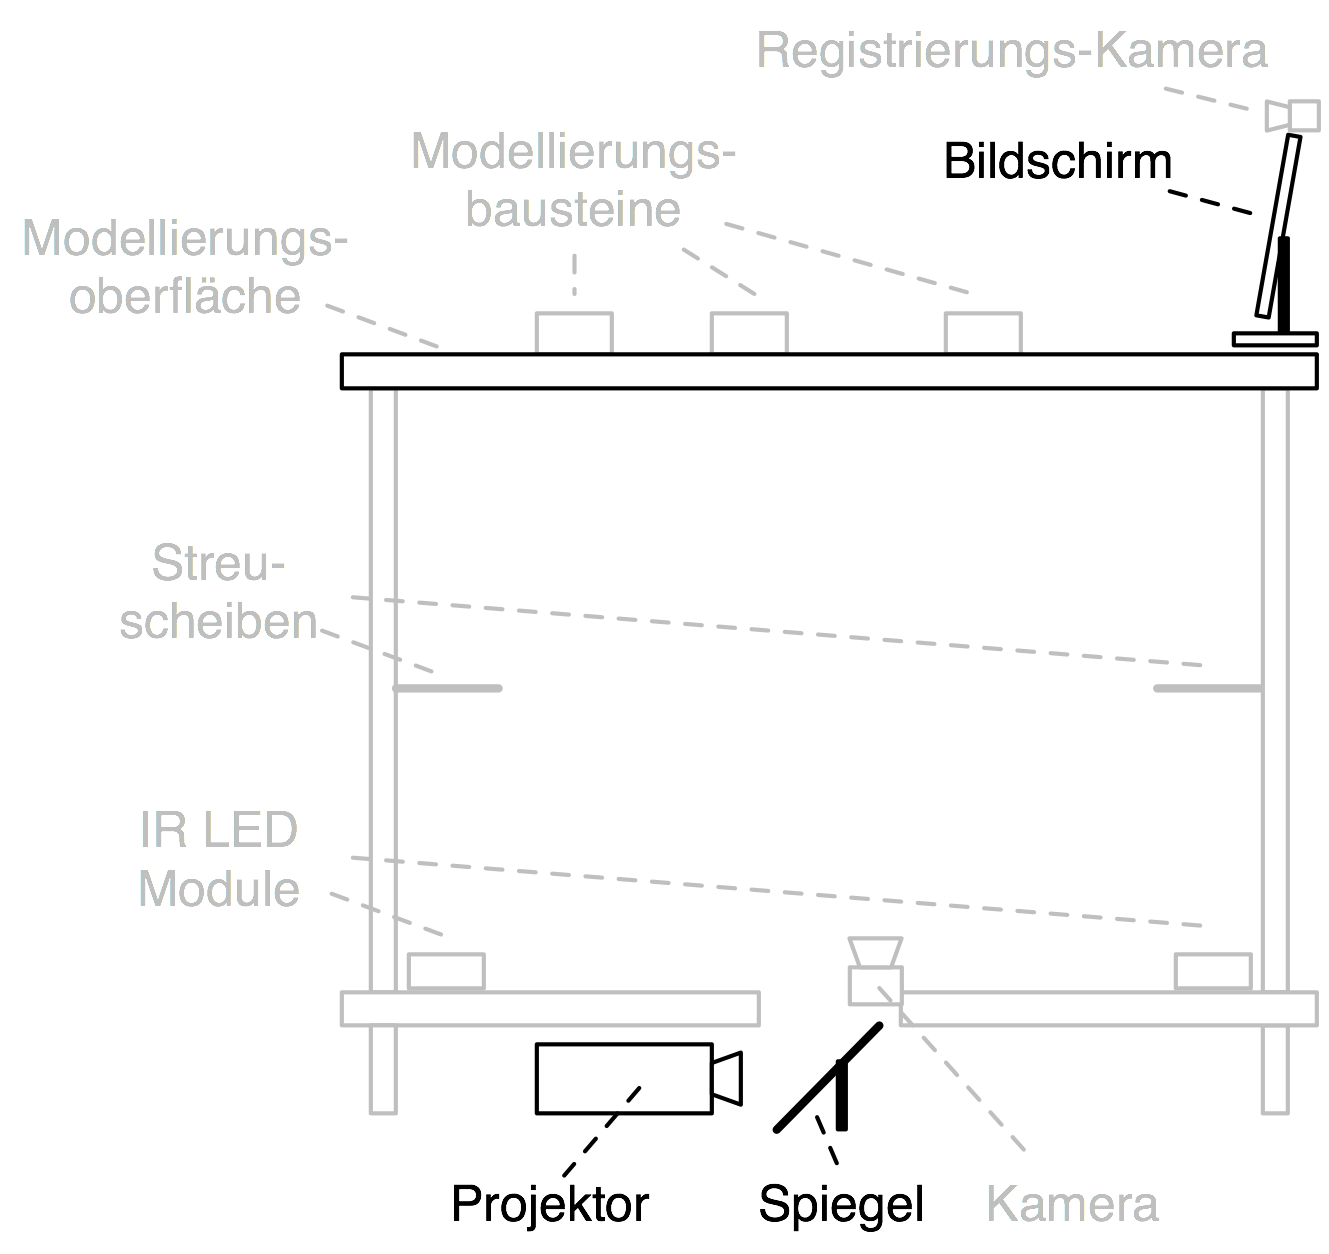
\includegraphics[height=3in]{img/ImplementierungInput/TischSeitenansichtOutput.png}
	\caption{Überblick über den Aufbau des Werkzeugs -- Ausgabekomponenten}
	\label{fig:img_ImplementierungInput_TischSeitenansichtOutput}
\end{figure}

% subsection output_ansatz_entscheidung (end)

\subsection{Frameworks zur Ausgabe} % (fold)
\label{sub:frameworks_zur_ausgabe}

Im Sinne der eben getroffenen Technologieentscheidung wird nun eine Softwarekomponente benötigt, die die Ansteuerung der Ausgabekanäle erlaubt. Diese Softwarekomponente muss im Wesentlichen die Modellinformation, die über die Eingabekanäle erhoben wurde, visuell ausgeben und zusätzlich den Modellierungsunterstützungs-Funktionen des Werkzeugs einen Kanal zur Kommunikation mit den Benutzern bieten.

Für die graphische Darstellung diagrammatischer Modelle (also vernetzter Strukturen) existieren verschiedene Frameworks die -- basierend auf unterschiedlichen technologischen Ansätzen -- die Darstellung von Modellelementen, der Verbindung und der Manipulation des Modells durch bereits implementierte Funktionalität ermöglichen und unterstützen. 

\subsubsection{In Frage kommende Frameworks} % (fold)
\label{ssub:in_frage_kommende_frameworks}

--> JHotDraw + evtl. andere Frameworks aus KnowIT-Diplomarbeit

\paragraph{JHotDraw} % (fold)
\label{par:jhotdraw}

Das JHotDraw-Framework (REF Gamma) ist eine Java-Implementierung des Smalltalk-Frameworks HotDraw (REF). Dieses wurde entwickelt, um einerseits eine einfache Möglichkeit zur Erstellung graphischer Editoren beliebiger Natur zu bieten und andererseits die Stärken und Möglichkeiten objektorientierter Softwareentwicklung unter Einsatz der von (REF Entwurfsmuster) vorgeschlagenen Entwurfsmuster zu zeigen.

JHotDraw nutzt intensiv objektorientierte Konzepte, vorallem die dynamische Typisierung von Objekten und implementiert einen Großteil seiner Features als Instanzen der eben erwähnten Entwurfsmuster. Dies erleichtert die Adaptierung und Erweitungerung des Systems für eigenen Anwendungsfälle und ermöglicht eine rasche, unaufwändige Implementierung anwendungsspezifischer graphischer Editoren.

% paragraph jhotdraw (end)

\subsubsection{Framework-Entscheidung} % (fold)
\label{ssub:output:framework_entscheidung}

% subsubsection output_framework_entscheidung (end)
% subsubsetion in_frage_kommende_frameworks (end)

% subsection subsection_name (end)
% subsubsection jhotdraw (end)

% subsection frameworks_zur_ausgabe (end)

% section technologische_grundlage_der_visualisierung (end)

\section{Ausgabe von Information} % (fold)
\label{sec:ausgabe_von_information}

In diesem Abschnitt wird nun auf Basis der eben getroffenen Framework-Entscheidung und unter Berücksichtigung der grundsätzlichen Entscheidung für zwei Ausgabekanäle, die in Abschnitt \ref{sec:technologische_grundlage_der_visualisierung} getroffen wurde, die konkrete Informationsausgabe für das hier vorgestellte Werkzeug beschrieben.

Wiederum auf abstrakter Ebene beginnend, wird das Konzept beschrieben, das bei der Umsetzung der Ausgabe verfolgt wird. Aufbauend darauf wird die Architektur der Software beschrieben, die auf den im letzten Kapitel beschriebenen Komponenten aufsetzt und für die Ansteuerung der Ausgabekanäle sorgt. Nach einer detaillierten Beschreibung der konkreten Ausgabeform für alle ausgebenden Informationstypen wird schließlich die Implementierung des hier verfolgten Ansatzes in Software vorgestellt.

\subsection{Konzept} % (fold)
\label{sub:ausgabe_konzept}

Wie bereits oben beschrieben wird die auszugebende Information im konkreten Werkzeug auf zwei Ausgabekanäle verteilt. Grundsätzlich wird Information auf einem mit den Eingabekanälen räumlich kohärenten Kanal (der Tischoberfläche) ausgegeben. Ist dies aufgrund der Art der auszugebenden Information nicht adäquat möglich, wird der zweite Ausgabekanal als primäres Kommunikationsmedium verwendet. In der übrigen Zeit spielt der zweite Ausgabekanal eine untergeordnete Rolle und kann zur unterstützenden simulatenen Visualisierung der am primären Kanal ohnehin ausgegebenen Information dienen.

Während eines Modellierungsvorgangs bleibt der Fokus der Ausgabe grundsätzlich am primären Ausgabekanal, der Tischoberfläche, auf der kohärent mit den auf ihr platzierten Tokens Information ausgegeben wird. In lediglich zwei Fällen erhält der zweite Ausgabekanal den Fokus:
\begin{itemize}
 \item Wenn Information ausgegeben werden muss, die nicht kohärent mit den auf der Oberfläche physischen Tokens dargestellt werden kann (z.B. bei der Ausgabe von gespeicherten Modellzuständen).
 \item Wenn Interaktion mit den Benutzern einen Fokus auf die digitale Welt, also auf über den Rechner zugreifbare Ressourcen hat (wie bei der Auswahl von Dateien zur Einbettung in Container-Tokens).
\end{itemize}
In beiden Fällen wird das Modell auf der Oberfläche nicht unmittelbar verändert, den Benutzern ist es möglich, sich auf die Interaktion mit dem sekundären Ausgabekanal zu konzentrieren.

Während der Arbeit mit dem Werkzeug, bei der der zweite Ausgabekanal grundsätzlich nicht benötigt wird, können zwei Ansätze verfolgt werden, was den Umgang mit diesem betrifft. Zum ersten kann der zweite Ausgabekanal abgeschaltet werden, also keine Ausgabe über den Bildschirm oder externen Projektor mehr erfolgen. Vorteil dieser Lösung ist, das ein Fokuswechsel auf den sekundären Ausgabekanal eindeutig erkennbar ist, da dazu die Darstellung explizit aktiviert werden muss. Während der eigentlichen Modellierung werden Benutzer nicht abgelenkt und können auf die Interaktion auf der Tischoberfläche fokussieren.

Zum zweiten ist es möglich, am sekundären Ausgabekanal die Ausgabe des primären Kanals zu spiegeln, auf diesem also synchron die gleiche Information auszugeben wie auf der Tischoberfläche. Ein Vorteil dieser Lösung ist, dass in dieser Darstellung zusätzlich Information eingeblendet werden kann, die auf der Tischoberfläche in der Überdeckung zwischen physischen Elementen und projizierter Information nicht dargestellt werden kann. So ist unter anderem denkbar, die Abstaktionsstufe, auf der aktuell modelliert wird, am sekundären Ausgabekanal zu visualisieren. Diese Information ist aus dem Modell auf der Tischoberfläche nicht erkennbar (weder eingebettete Teilmodelle noch übergeordnete Modelle sind auf im Modell ohne weitere Interaktion sichtbar), für den Modellierungsvorgang aber auch zumeist nicht unmittelbar relevant. Ist sie nun auf der sekundären Oberfläche permanent sichtbar, besteht für Benutzer die Möglichkeit, sich rasch und ohne zusätzlichen Interaktionsaufwand einen Überblick über den Kontext des aktuell bearbeiteten (Teil-)Modells zu erhalten.

Ein zweiter Aspekt der Spiegelung der Ausgabe auf dem sekundären Ausgabekanal ist das unmittelbare Feedback, das Benutzern über die Tätigkeit des Systems zur Verfügung gestellt wird. Wenn ein Modellierungstoken bewegt oder geöffnet wird, erfolgt eine unmittelbare Reaktion in der Modellvisualisierung auf dem sekundären Ausgabekanal. Auch eventuelle Fehlerkennungen werden offensichtlich, wenn z.B. ein Element von der sekundären Visualisierung verschwindet, obwohl es auf der Oberfläche noch vorhanden ist. Für Benutzer ist damit das Systemverhalten klarer erkennbar, die Bildung eines mentalen Modells zur Erklärung der Funktionsweise des Werkzeugs ist einfacher und lenkt nach der Einarbeitungsphase nicht mehr von der eigentlichen Tätigkeit ab (REF Norman Design of everyday things, Kühlschrankregelung). Letztendlich besteht bei der Einbindung mehrerer Benutzer die Möglichkeit, allen Beteiligten einen Überblick über den aktuellen Modellzustand zur Verfügung zu stellen auch wenn diese im Moment nicht aktiv am Werkzeug arbeiten. Nachteile dieses Ansatzes liegen einerseits in der möglichen Ablenkung der Benutzer von der eigentlichen Modellierungsoberfläche (was insofern weitgehend unkritisch ist, als das die gesamt Information über den sekundären Informationskanal zur Verfügung gestellt wird), vor allem aber darin, das der Wechsel des Interaktionsfokus von einem Ausgabekanal zum anderen nicht mehr so explizit sichtbar wird wie im ersten Ansatz. Benutzer sind so unter Umständen desorientiert und können dem Systemverhalten nicht folgen.

Aus den vorangegangenen Ausführungen ist ersichtlich, dass beide Ansätze Vor- und Nachteile bieten, die nicht eindeutig für eine der beiden Lösungen sprechen. Vielmehr muss im einzelnen Anwendungsfall abgewogen werden, welche Lösung eher geeignet ist. Einflussfaktoren sind dabei die Anzahl der an der Modellierung teilnehmenden Benutzer (bessere Verfolgbarkeit des Modellierungsvorgangs bei synchroner Anzeige auf beiden Kanälen), die Modellierungsaufgabe an sich (generelle Notwendigkeit der Nutzung des sekundären Ausgabekanals) sowie das persönliche Modellierungsverhalten der Beteiligten (eher am Bildschirm oder eher an der Tischoberfläche orientiert). Aus diesen Gründen werden beide Formen der Verwendung des sekundären Ausgabekanals unterstützt, wobei die Benutzer durch eine Tastenkombination zwischen den beiden Modi umschalten können -- also ggf. auch in unterschiedlichen Phasen eines Modellierungsvorgangs eine unterschiedliche Konfiguration der Ausgabekanäle nutzen können.

% subsection ausgabe_konzept (end)

\subsection{Architekur} % (fold)
\label{sub:architekur}

Wie im letzten Abschnitt beschrieben, unterscheidet sich die Ausgabe von Information auf den beiden Ausgabekanälen nur in einigen Fällen, im synchronen Ausgabemodus wird weitgehend die gleiche Information in -- den unterschiedlichen Ausgabemedien geschuldet -- zum Teil unterschiedlichen Ausgabeformen dargestellt.  

Grundsätzlich wird die Architektur der Ausgabekanal-Verwaltung erweiterbar angelegt, um veränderte Anforderungen an der Werkzeug oder erweiterte Funktionalität umsetzen zu können. Basis dieser erweiterbaren Architektur ist das in Abschnitt \ref{sub:verteilung_des_modellzustandes} bereits beschriebene Modul zur Verteilung des aktuellen Modellzustandes an die verwendeten Ausgabekanäle. Jeder Ausgabekanal, der über Änderungen am Modell an den Eingabekanälen benachrichtigt werden soll, muss ein definiertes Interface implementieren, das jene Methoden definiert, die zur Datenübermittlung zwischen dem Interpretationsmodul und den Ausgabekanälen notwendig sind. In der konkreten Implementierung sind zur Zeit zwei auf JHotDraw basierende Ausgabekanäle umgesetzt, zusätzlich existiert ein weiteres Modul, das gegenüber dem System als Ausgabekanal agiert, die übermittelte Information selbst jedoch wieder an beliebige via \gls{TCP}/\gls{IP} erreichbare Clients verteilt (siehe Abbildung \ref{fig:img_ImplementierungOutput_OutputArchitecture}). Auf diesem Weg können entfernte Ausgabekanäle realisiert werden, die es erlauben, den Modellierungsprozess auch ohne räumliche Anwesenheit zur verfolgen. Mittels der gleichen Schnittstelle können auch weitere, nicht auf visuelle Ausgabe beschränkte Kanäle wie z.B. akustische Benachrichtigungen mit Information versorgt werden. 

\begin{figure}[htbp]
	\centering
		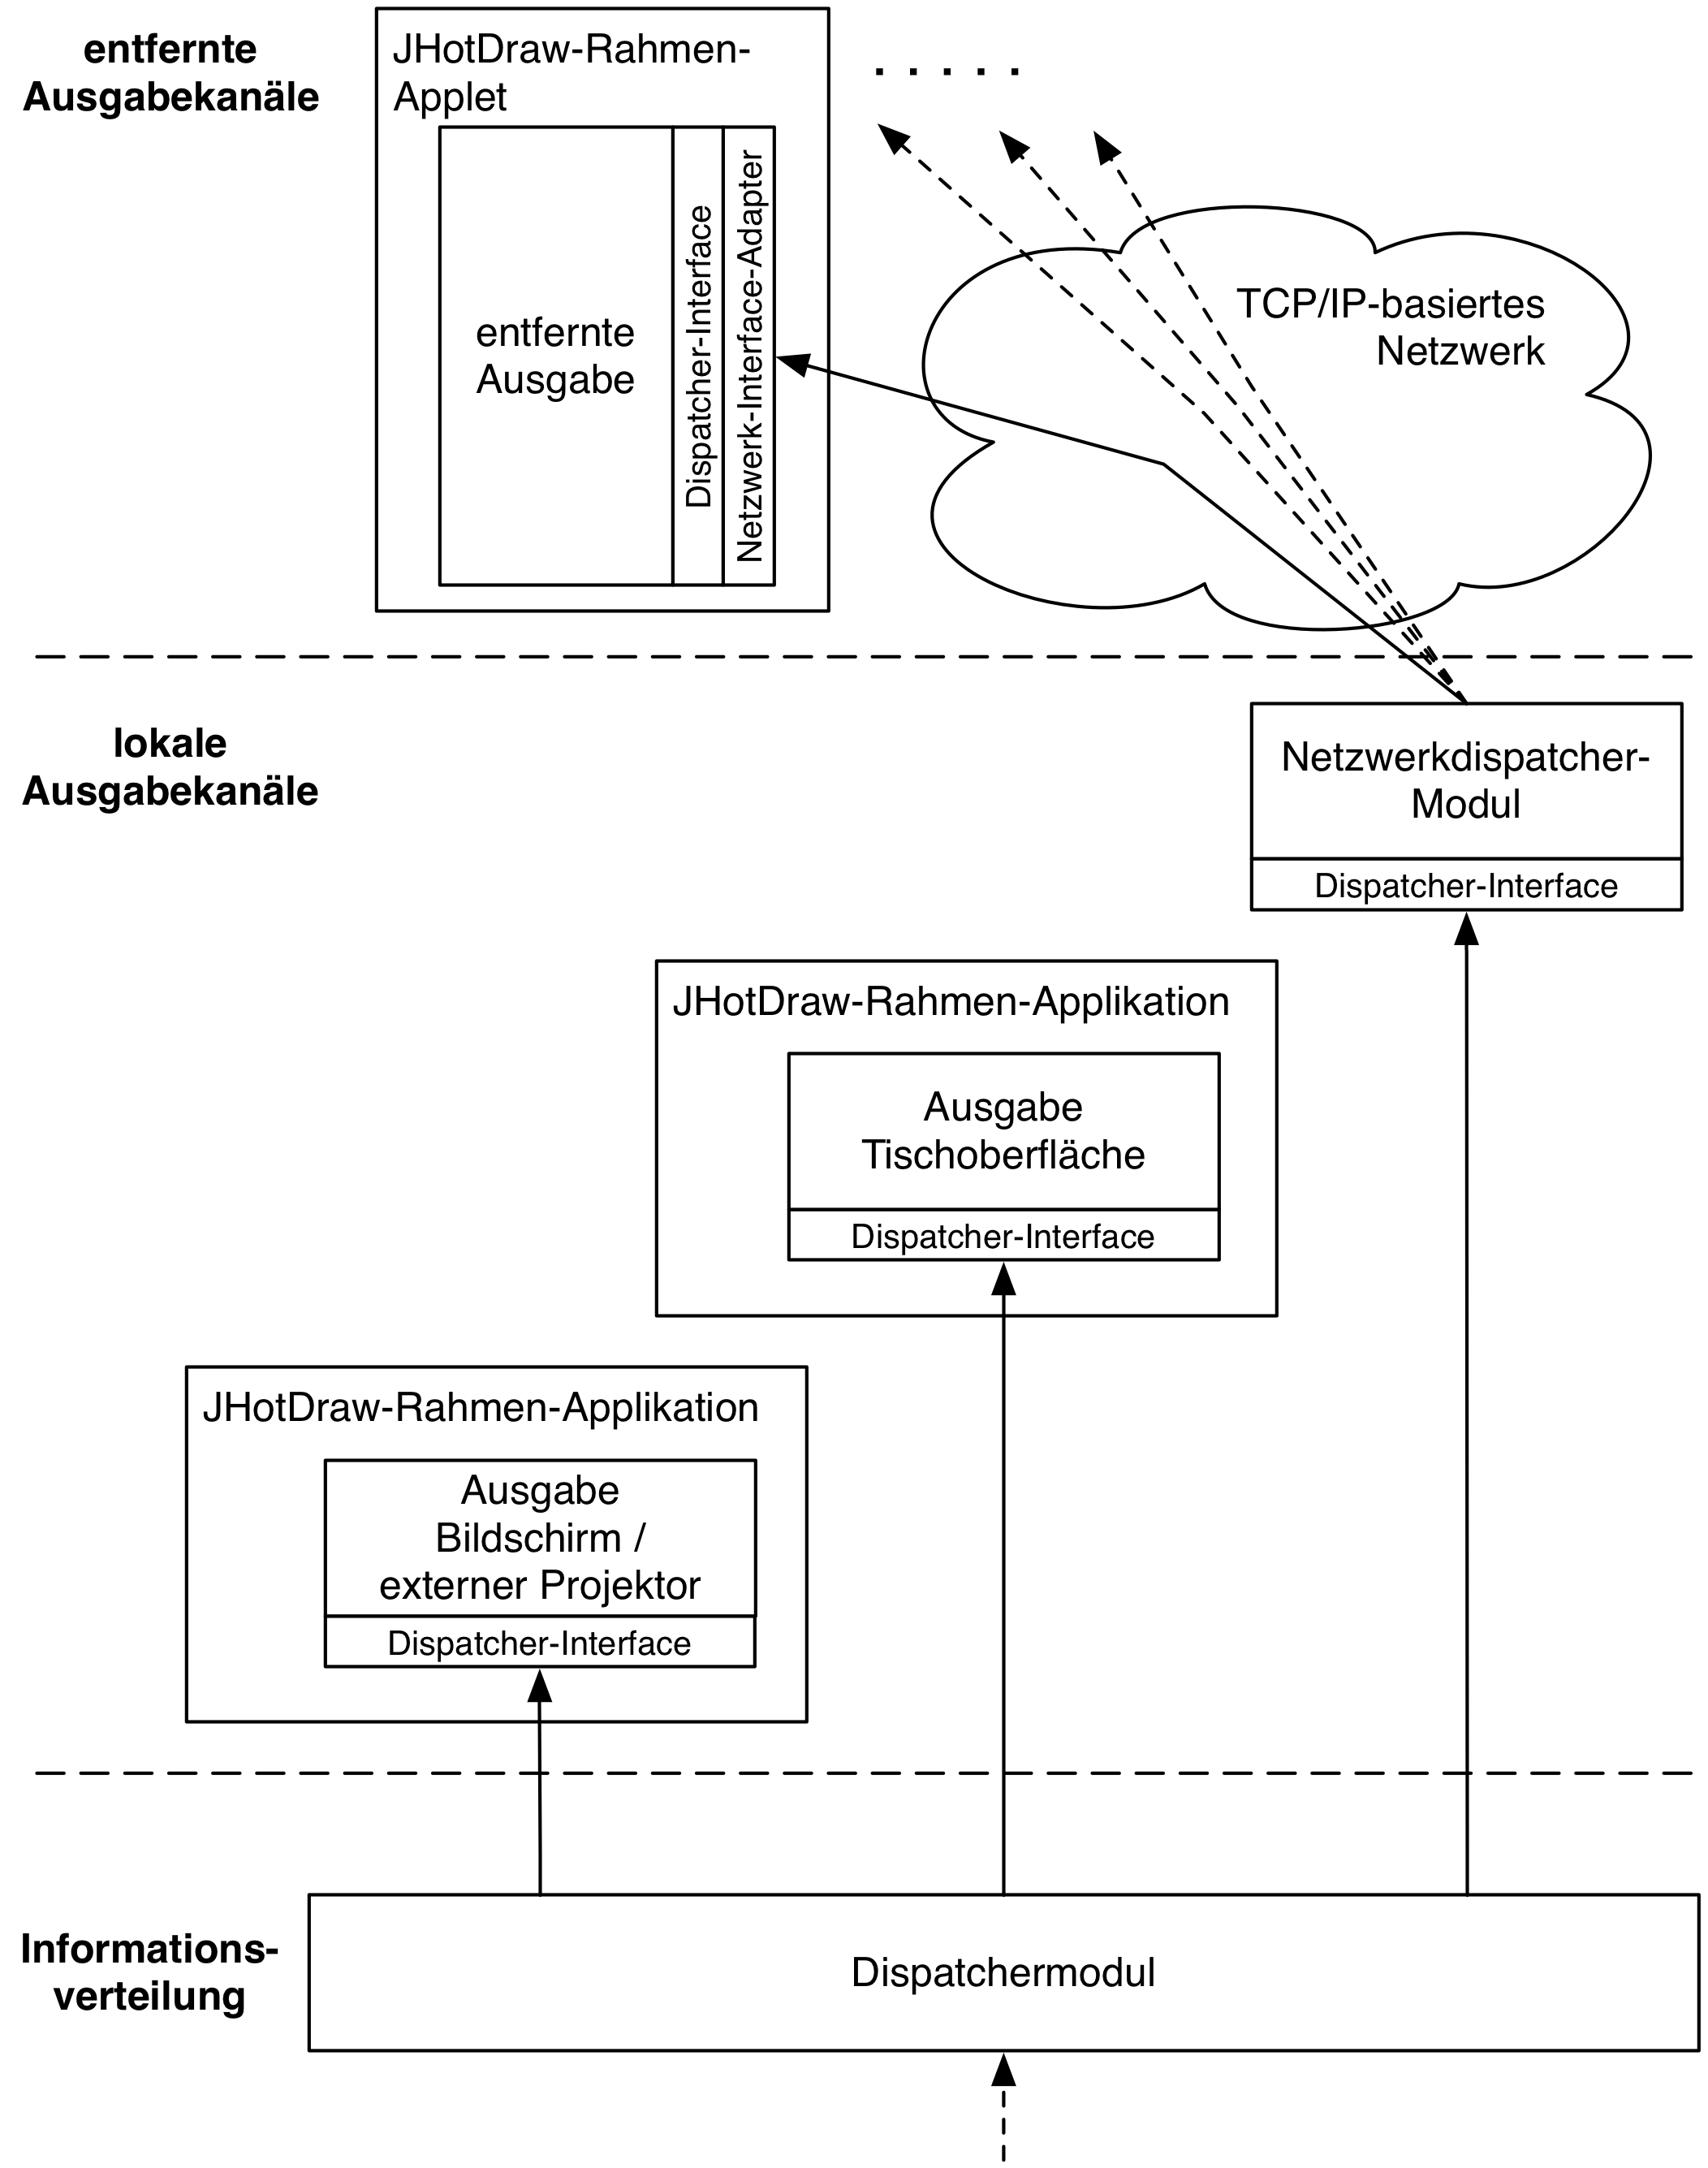
\includegraphics[width=15cm]{img/ImplementierungOutput/OutputArchitecture.png}
	\caption{Softwarearchitektur zur Verwaltung der Ausgabekanäle}
	\label{fig:img_ImplementierungOutput_OutputArchitecture}
\end{figure}

Durch die flexible Architekur von JHotDraw ist es möglich, unterschiedliche Ausgabekanäle mit der gleichen Codebasis durch den Einsatz verschiedener Basisklassen als vollständig eigenständige Applikation auszuführen oder als Applet in Webbrowsern zu starten (siehe Abbildung \ref{fig:img_ImplementierungOutput_OutputClasses}). Auf diese Weise ist es möglich, die einmal implementierte Visualisierung des Modellzustandes für die lokalen Ausgabekanäle sowie für entfernte Betrachter zu verwenden, die alle über die gleiche Schnittstelle synchron mit Information versorgt werden.

\begin{figure}[htbp]
	\centering
		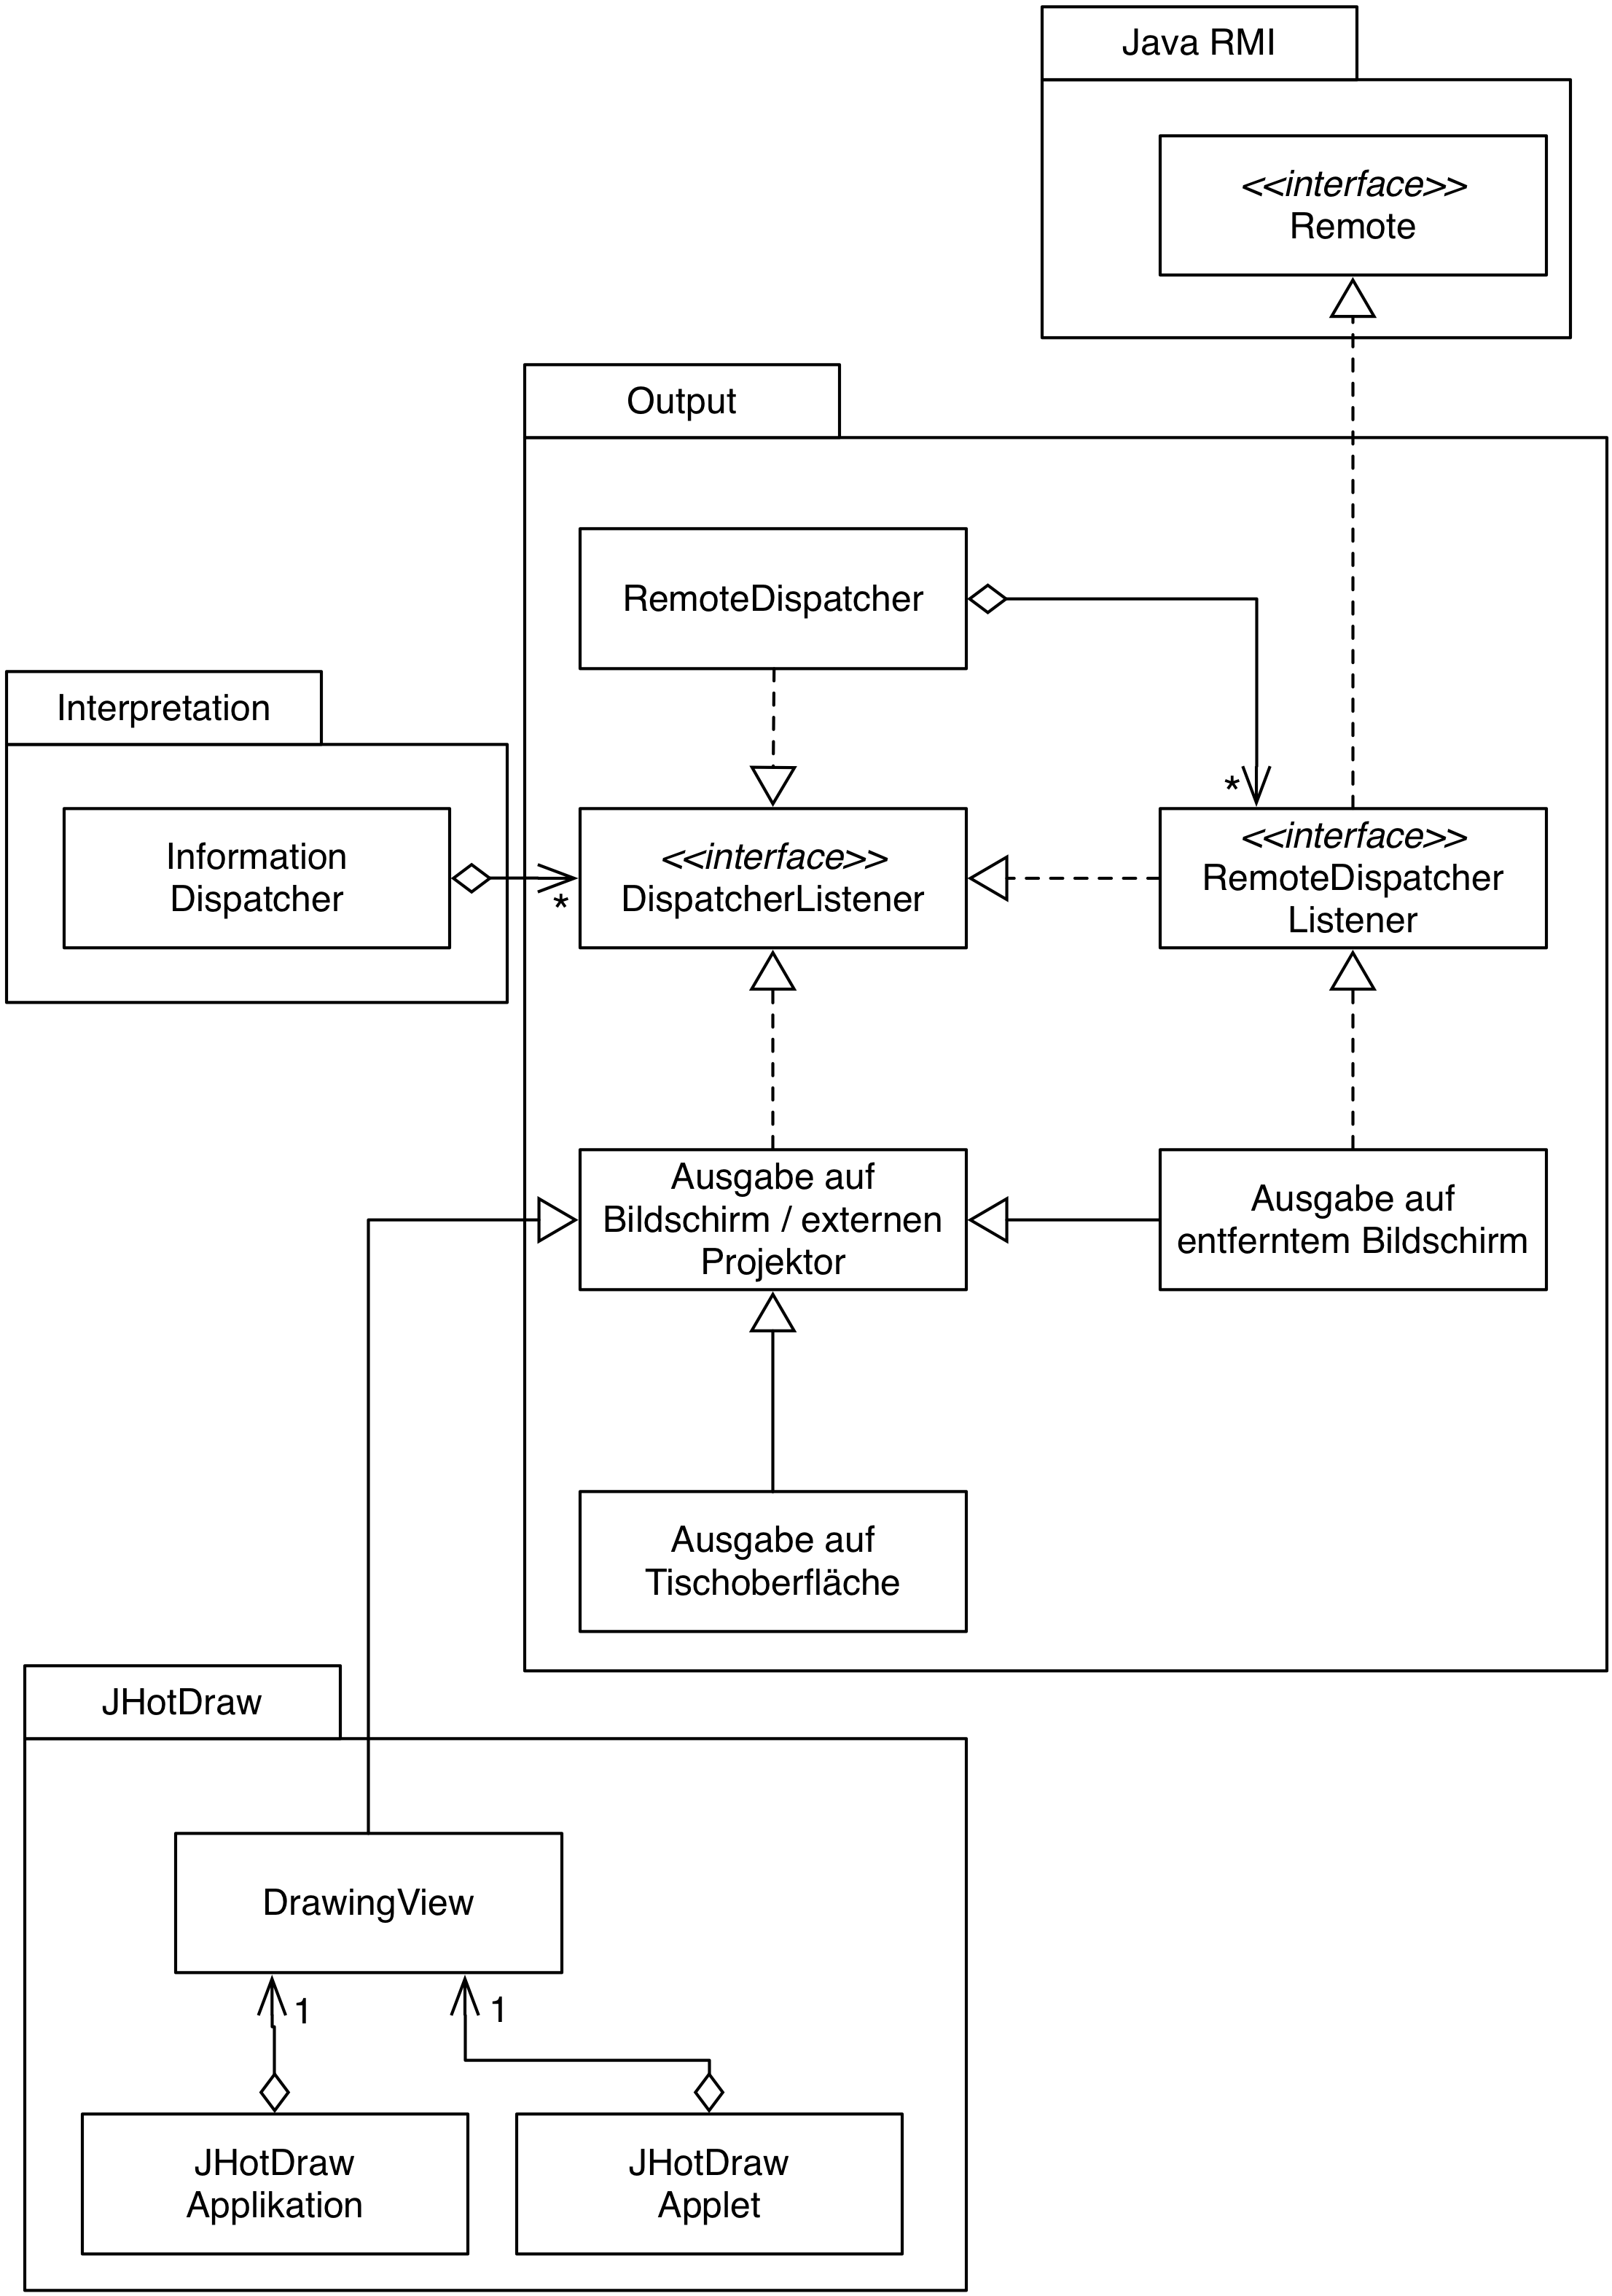
\includegraphics[width=13cm]{img/ImplementierungOutput/OutputClasses.png}
	\caption{Zusammenhänge der Klassen zur Ausgabebehandlung}
	\label{fig:img_ImplementierungOutput_OutputClasses}
\end{figure}

Die beiden lokalen Ausgabekanäle basieren wie bereits erwähnt auf einer einheitlichen Codebasis, die sich aufgrund der unterschiedlichen Anforderung jedoch in Detail der Darstellung unterscheidet. So müssen auf dem bildschirmbasierten Ausgabekanal unter anderem die Modellelemente graphisch dargestellt werden, wohingegen diese auf der Tischoberfläche in Form der physischen Modellierungstokens bereits vorhanden sind. Beiden Kanälen einheitlich ist hingegen zum Beispiel die Behandlung der Verbinder, die hier wie dort dargestellt werden müssen. Durch das nur partiell unterschiedliche Verhalten der beiden Ausgabekanäle ist es möglich, diese von einer gemeinsamen Basisklasse abzuleiten und die Spezifika in Subklassen zu imlementieren. Dies reduziert auch den Wartungsaufwand der Codebasis und vermindert die Gefahr von Inkonsistenzen.  
% subsection architekur (end)

\subsection{Ausgabe von Information zum Modell} % (fold)
\label{sub:ausgabe_von_information_zum_modell}

Um im Folgenden auf die Details der Implementierung eingehen zu können, muss an dieser Stelle noch ausgeführt werden, welche Arten von Information in welcher Form über welchen Kanal ausgegeben werden. Grundsätzlich sind konzeptuell zwei Arten von Information zu unterscheiden. Dieser Abschnitt behandelt die Ausgabe von Information zum Modell selbst, im folgenden Abschnitt werden jene Informationen Ausgabekanälen zugeordnet, die der Kontrolle des Systems und der Unterstützung des Modellierungsvorgangs dienen.

\subsubsection{Information zu Modellelementen} % (fold)
\label{ssub:information_zu_modellelemeenten}

Information, die im Zusammenhang mit einzelnen Modellelementen ausgegeben wird, wird unmittelbar auf der Modellierungsoberfläche, also am primären Ausgabekanal, dargestellt. Wenn der sekundäre Ausgabekanal für synchrone Modelldarstellung konfiguriert ist oder entfernte Modellbetrachter eingesetzt werden, so wird diese Information auch auf diesen dargestellt, wobei die Ausgabe auf diesen identisch ist (dies gilt auch in den weiteren Abschnitten). Dabei wird das Modellelement selbst graphisch repräsentiert, um eine Zuordnung der Information zu ermöglichen. Auf der Tischoberfläche ist eine dezidierte Darstellung des Modellelements nicht notwendig, das dieses durch die kohärente Eingabe ohnedies durch das entsprechende Modellierungstoken dargestellt wird (siehe Abbildung \ref{fig:img_SystemNeu_Token})

\begin{figure}[htbp]
	\centering
		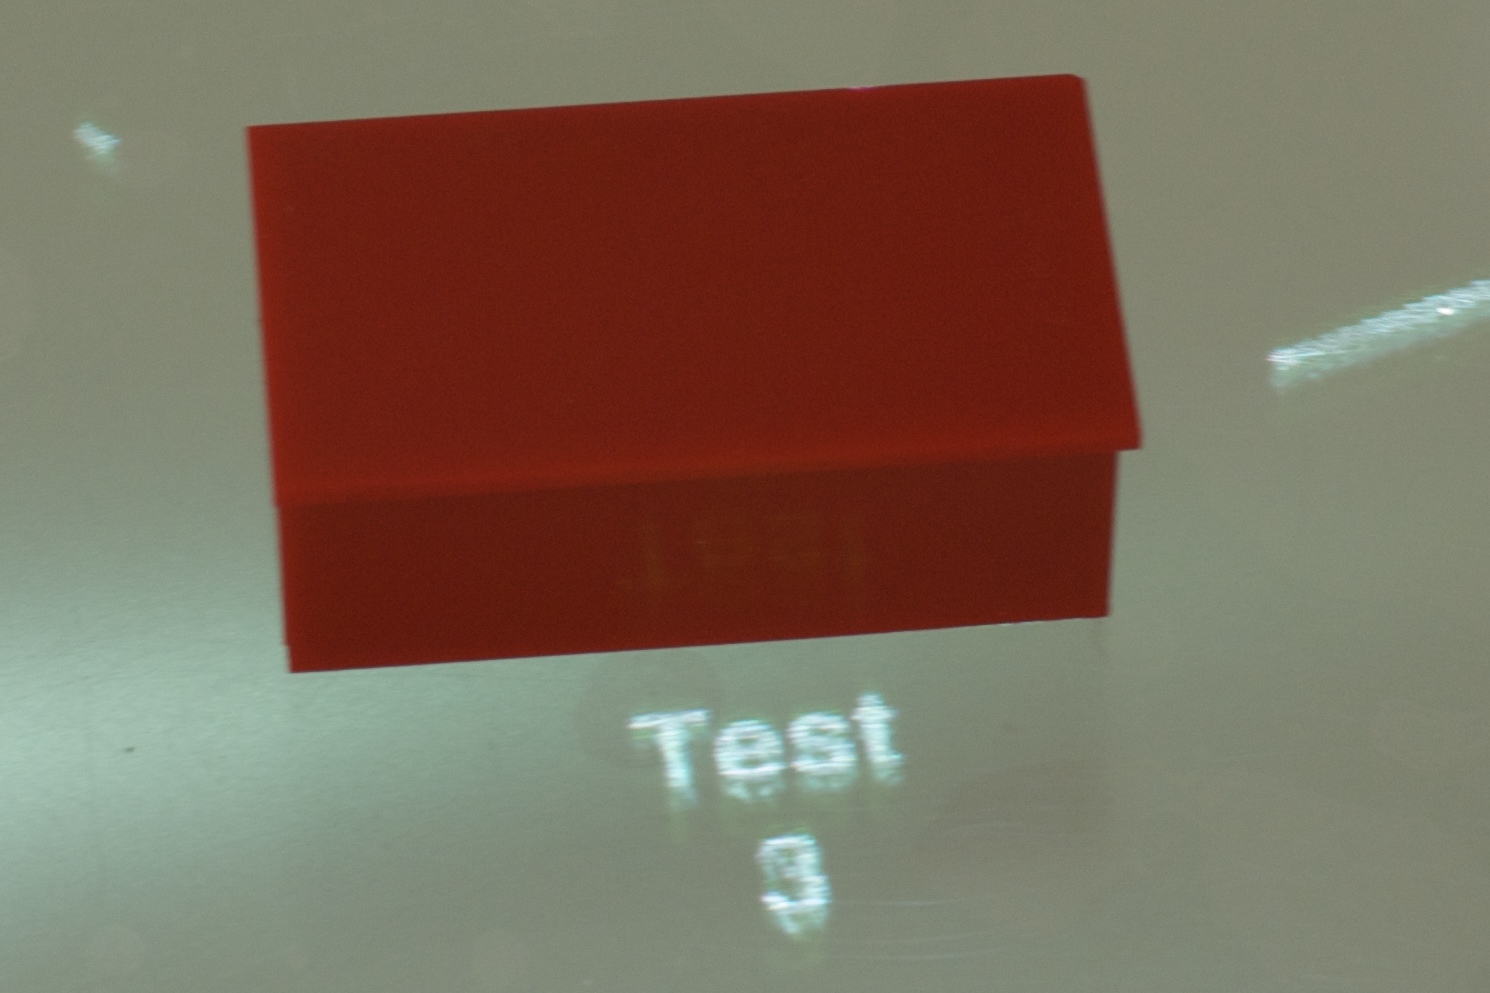
\includegraphics[width=5cm]{img/SystemNeu/TokenTisch.jpg}
		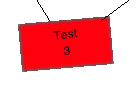
\includegraphics[width=5cm]{img/SystemNeu/TokenScreen.png}
	\caption[Darstellung von Modellelementen]{\centering Darstellung von Modellelementen \par \centering (links: Tischoberfläche, rechts: Bildschirm)}
	\label{fig:img_SystemNeu_Token}
\end{figure}

In der aktuellen Implementierung wird an Information lediglich die Bezeichnung des Tokens auf beiden Ausgabekanälen explizit ausgegeben. Der Typ des Tokens ist in der Farb- und Formgebung codiert.  Auf dem sekundären Ausgabekanal ist sind die Elemente in der graphischen Darstellung den physischen Elementen nachempfunden und bilden deren Farbe und Grundriss ab.

Ebenfalls nur auf der sekundären Oberfläche explizit auszugeben ist die Information hinsichtlich der aktuellen Rotation eines Modellierungstokens. Auf der Oberfläche ist diese am physischen Token erkennbar bzw. wird durch diese festgelegt. In der graphischen Repräsentation am sekundären Ausgabekanal muss diese Rotation ebenfalls abgebildet und nachgeführt werden.

% subsubsection information_zu_modellelementen (end)

\subsubsection{Information zu Verbindern} % (fold)
\label{ssub:information_zu_verbindern}

Da Verbinder nicht physisch existieren sondern immer über die Ausgabekanäle dargestellt werden müssen, gelten die nun folgenden Ausführungen für beide Ausgabekanäle. Wird ein Verbinder hergestellt, so kann neben den beiden Endpunkten (Modellelementen) auch noch die Richtung des Verbinders sowie eine Bezeichnung festgelegt werden.

\begin{figure}[htbp]
	\centering
		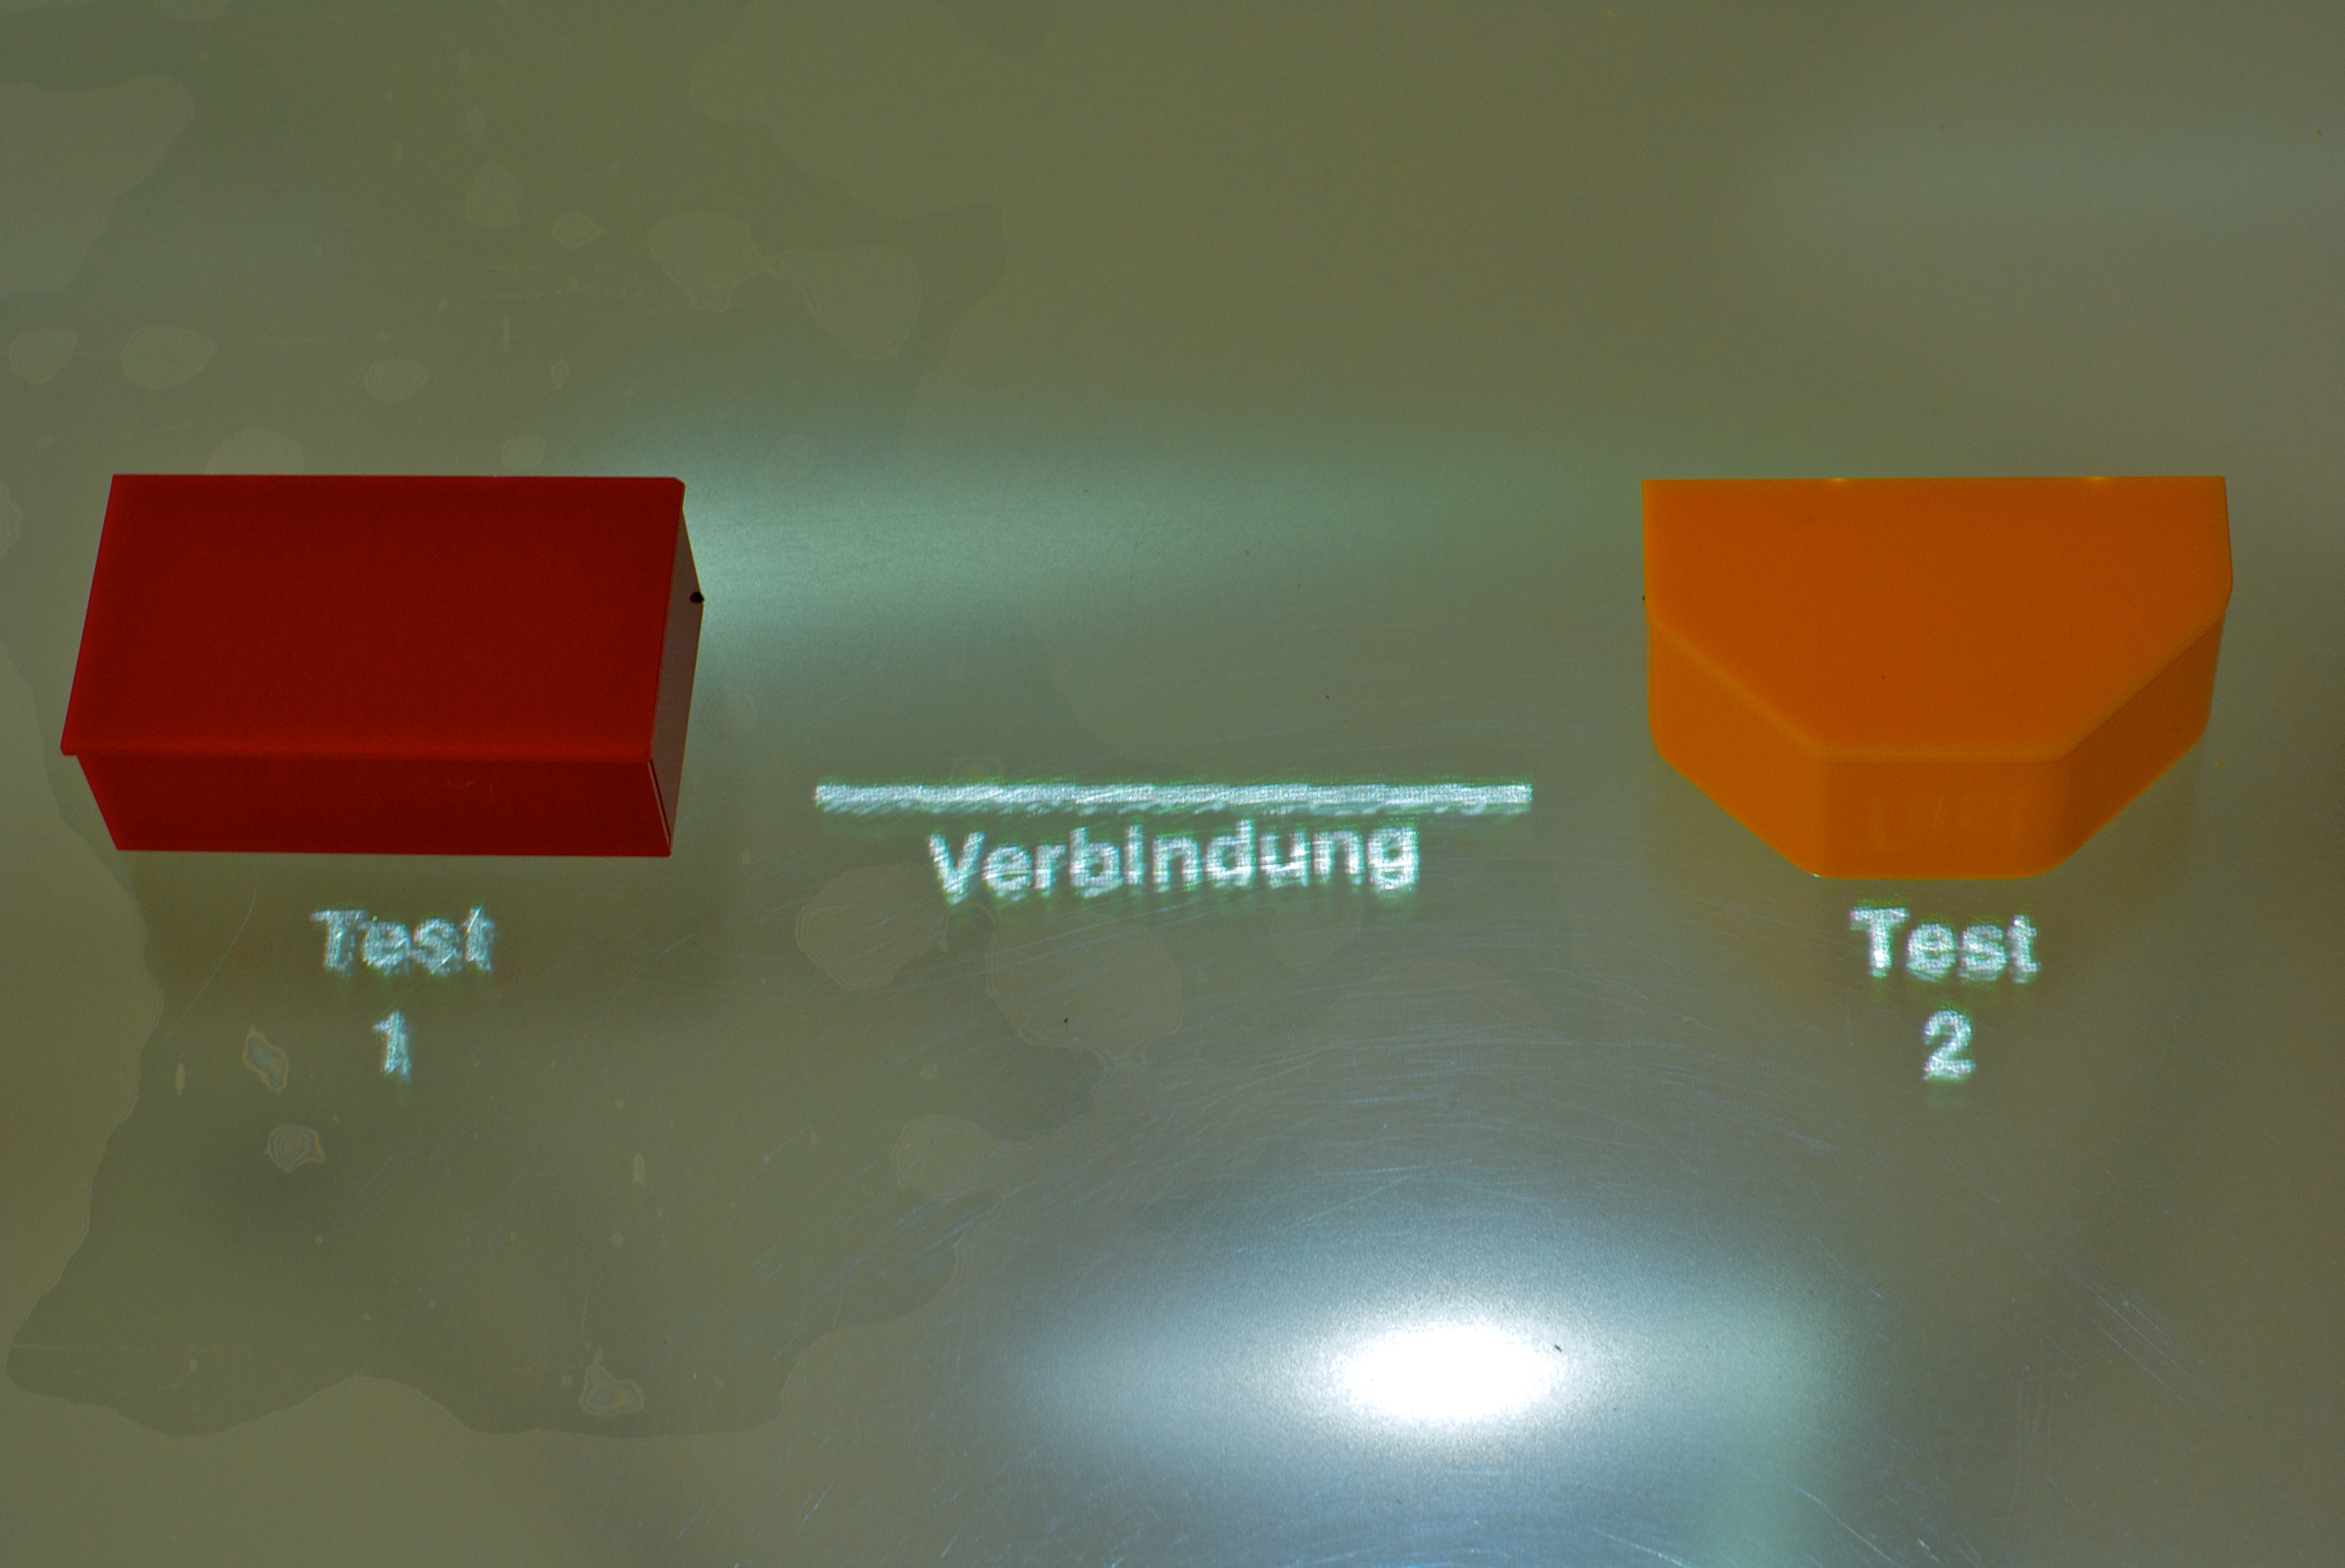
\includegraphics[height=2in]{img/SystemNeu/VerbindungTisch.jpg}
		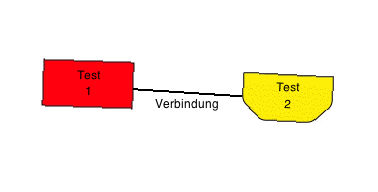
\includegraphics[height=2in]{img/SystemNeu/VerbindungScreen.png}
	\caption[Darstellung von Verbindern]{\centering Darstellung von Verbindern \par \centering (oben Tischoberfläche, unten Bildschirm)}
	\label{fig:img_SystemNeu_Verbinder}
\end{figure}

Ein Verbinder wird auf den Ausgabekanälen als Linie dargestellt die zwei Modellierungstokens bzw. deren graphische Repräsentation verbindet (siehe Abbildung \ref{fig:img_SystemNeu_Verbinder}). Die Richtung des Verbinders wird über Pfeilspitzen angegeben, die an den Enden der Linien angebracht werden (siehe Abbildung \ref{fig:img_SystemNeu_VerbindungGerichtetTisch}). Dabei können diese Pfeilspitzen fehlen (ungerichteter Verbinder), an einem Ende angebracht werden (gerichteter Verbinder) oder an beiden Enden dargestellt werden (bidirektionaler Verbinder). Die Ausgabe der Benennung eines Verbinders erfolgt -- sofern vorhanden -- zentriert auf halbem Weg zwischen den verbundenen Modellelementen unterhalb der Linie. 

\begin{figure}[htbp]
	\centering
		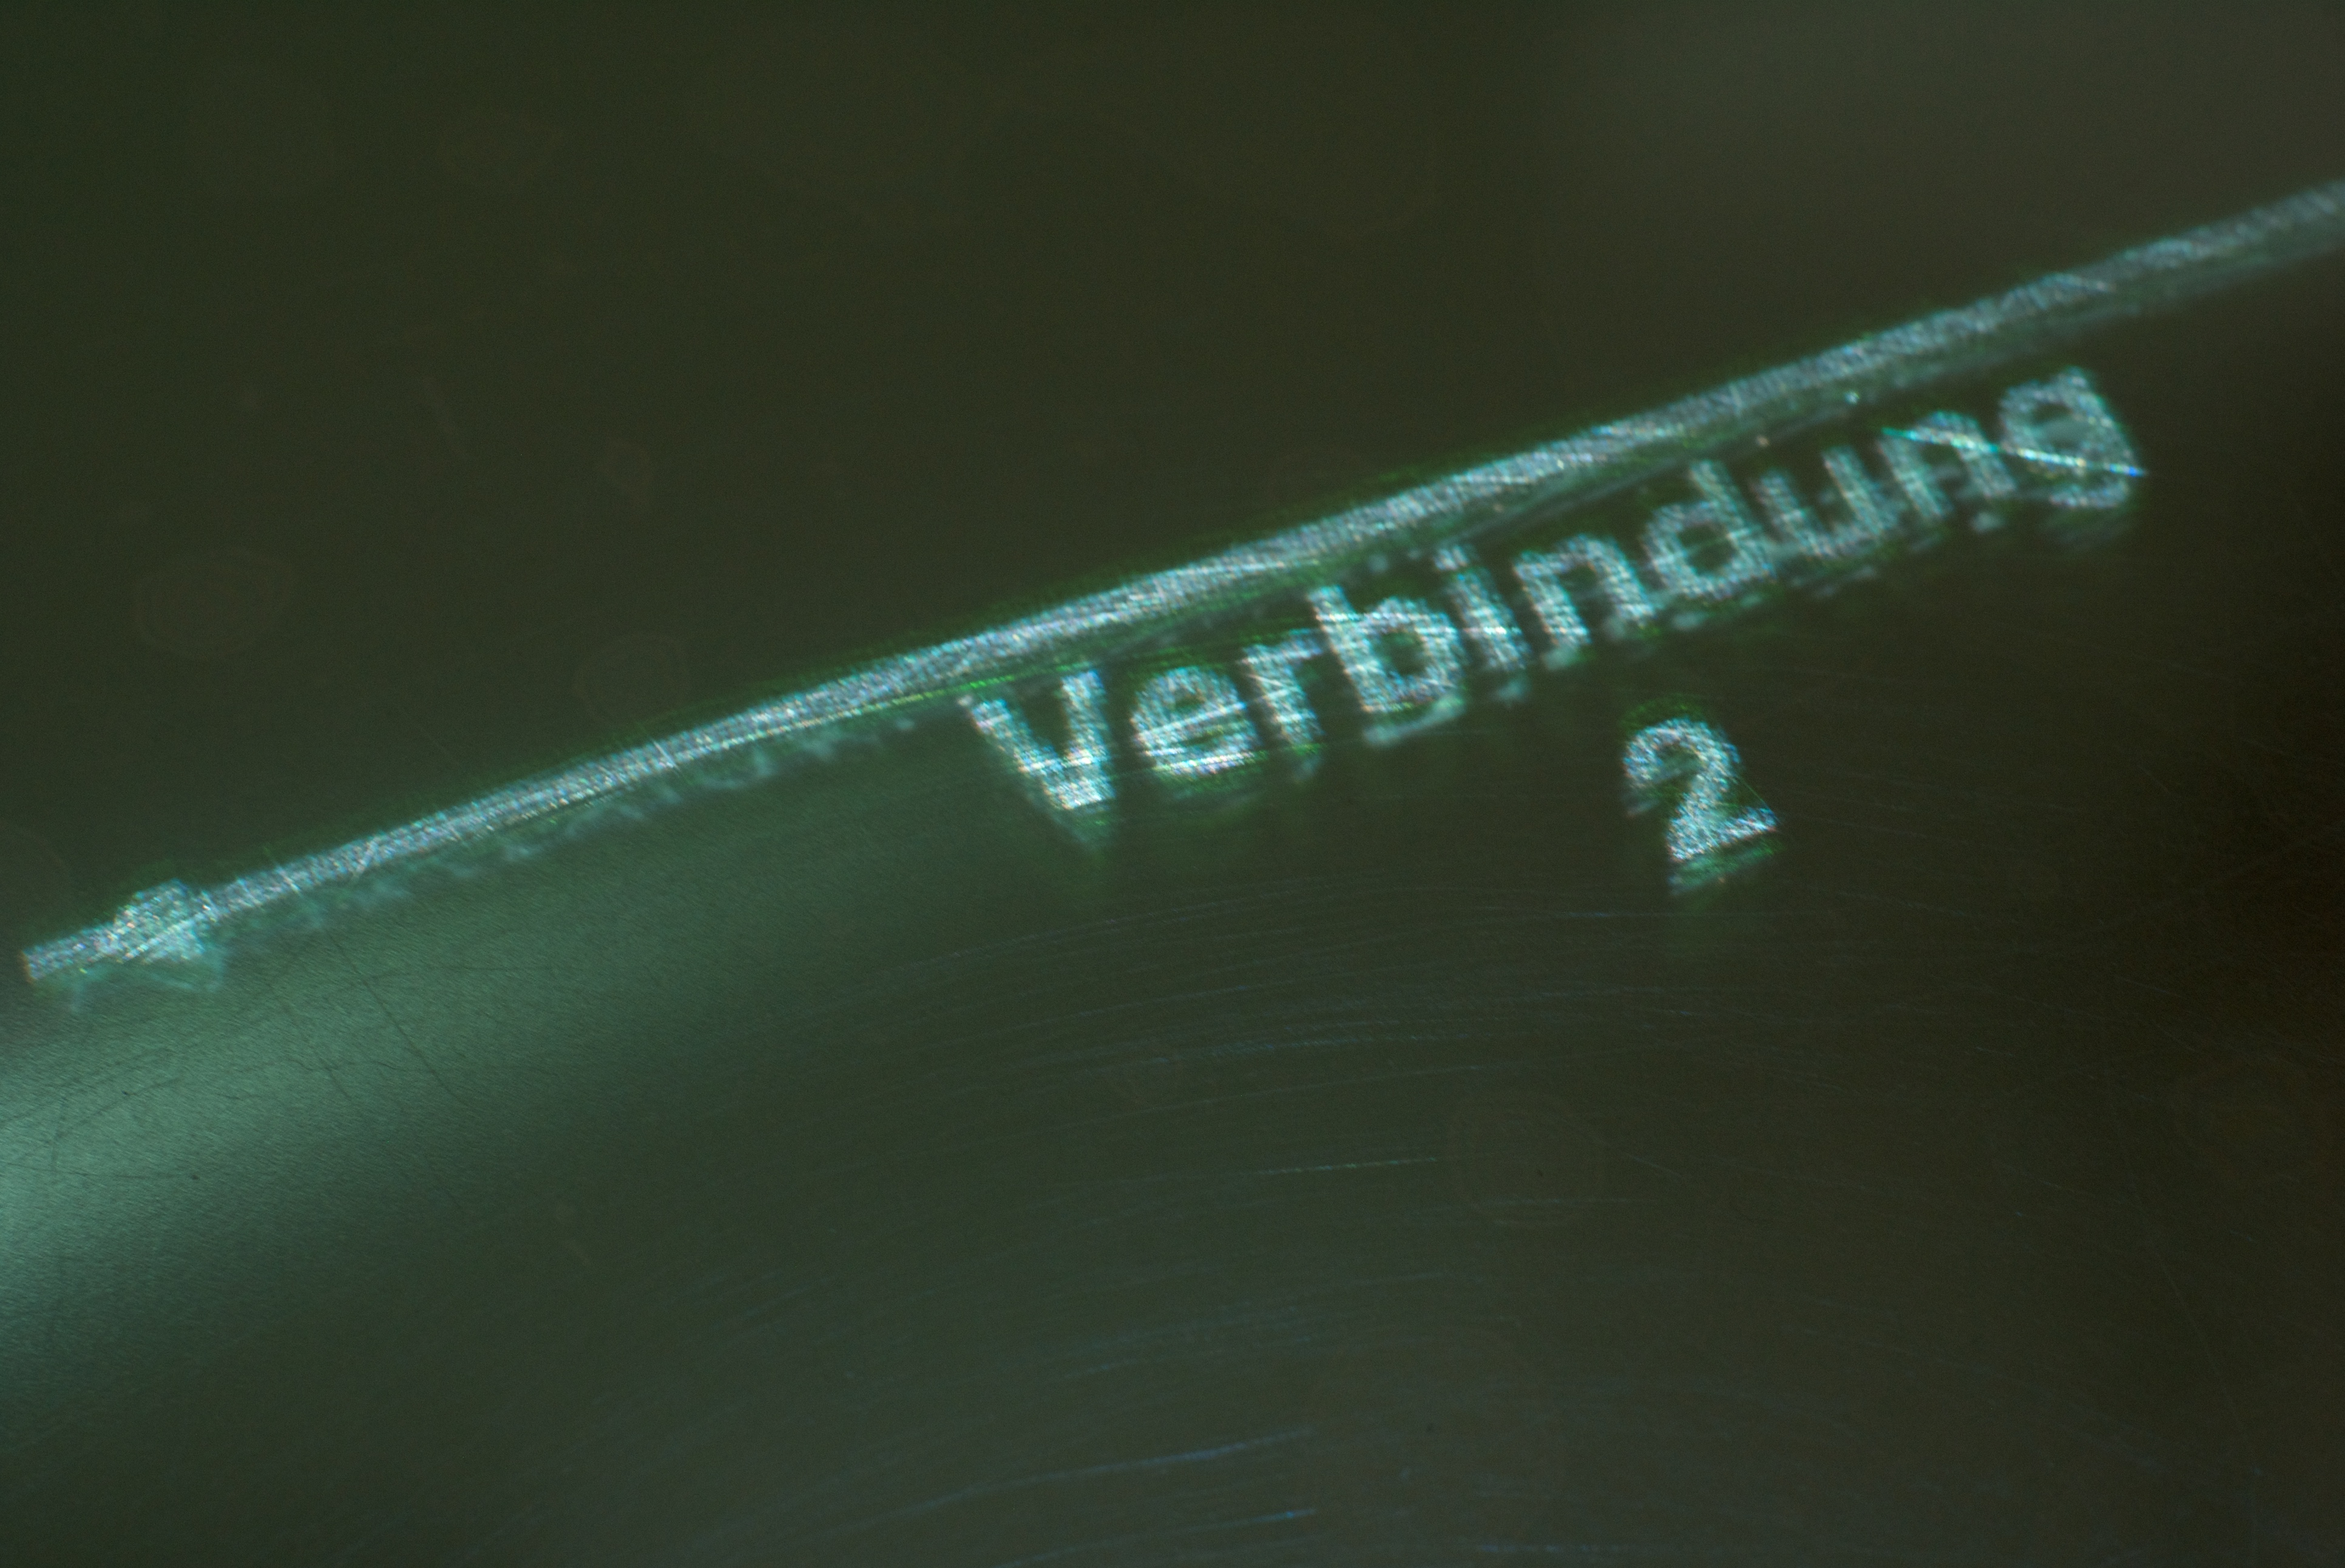
\includegraphics[height=2in]{img/SystemNeu/VerbindungGerichtetTisch.jpg}
	\caption{Darstellung gerichteter Verbinder}
	\label{fig:img_SystemNeu_VerbindungGerichtetTisch}
\end{figure}

% subsubsection information_zu_verbindern (end)

\subsubsection{Information zu eingebetteten Elementen} % (fold)
\label{ssub:information_zu_eingebetteten_elementen}
% subsubsection information_zu_eingebetteten_elementen (end)

Im Kontext der Ausgabe von Information zu eingebetteten Elementen müssen unterschiedliche Modellaspekte berücksichtigt werden. Im einzelnen sind dies:
\begin{itemize}
 \item Öffnungszustand von Modellelementen
 \item Anzahl und Art der eingebetteten Elemente
 \item Information, welche an eingebettete Elemente gebunden ist
\end{itemize}

Der Öffnungszustand von Modellelementen ist auf der Tischoberfläche durch den Zustand des jeweiligen Containertokens ersichtlich. Auch die Art und Anzahl der eingebetteten Elemente ist sichtbar, wenn ein Containertoken geöffnet ist. Am sekundären Ausgabekanal, also auf dem Bildschirm wird ein geöffnetes Modellelement vergrößert dargestellt, um innerhalb der Fläche des Elements visuelle Repräsentationen der eingebetteten Elemente einblenden zu können. Somit ist auch am sekundären Ausgabekanal erkennbar, wann bzw. dass ein Element geöffnet ist (siehe Abbildung \ref{fig:img_SystemNeu_Container}). 

\begin{figure}[htbp]
	\centering
		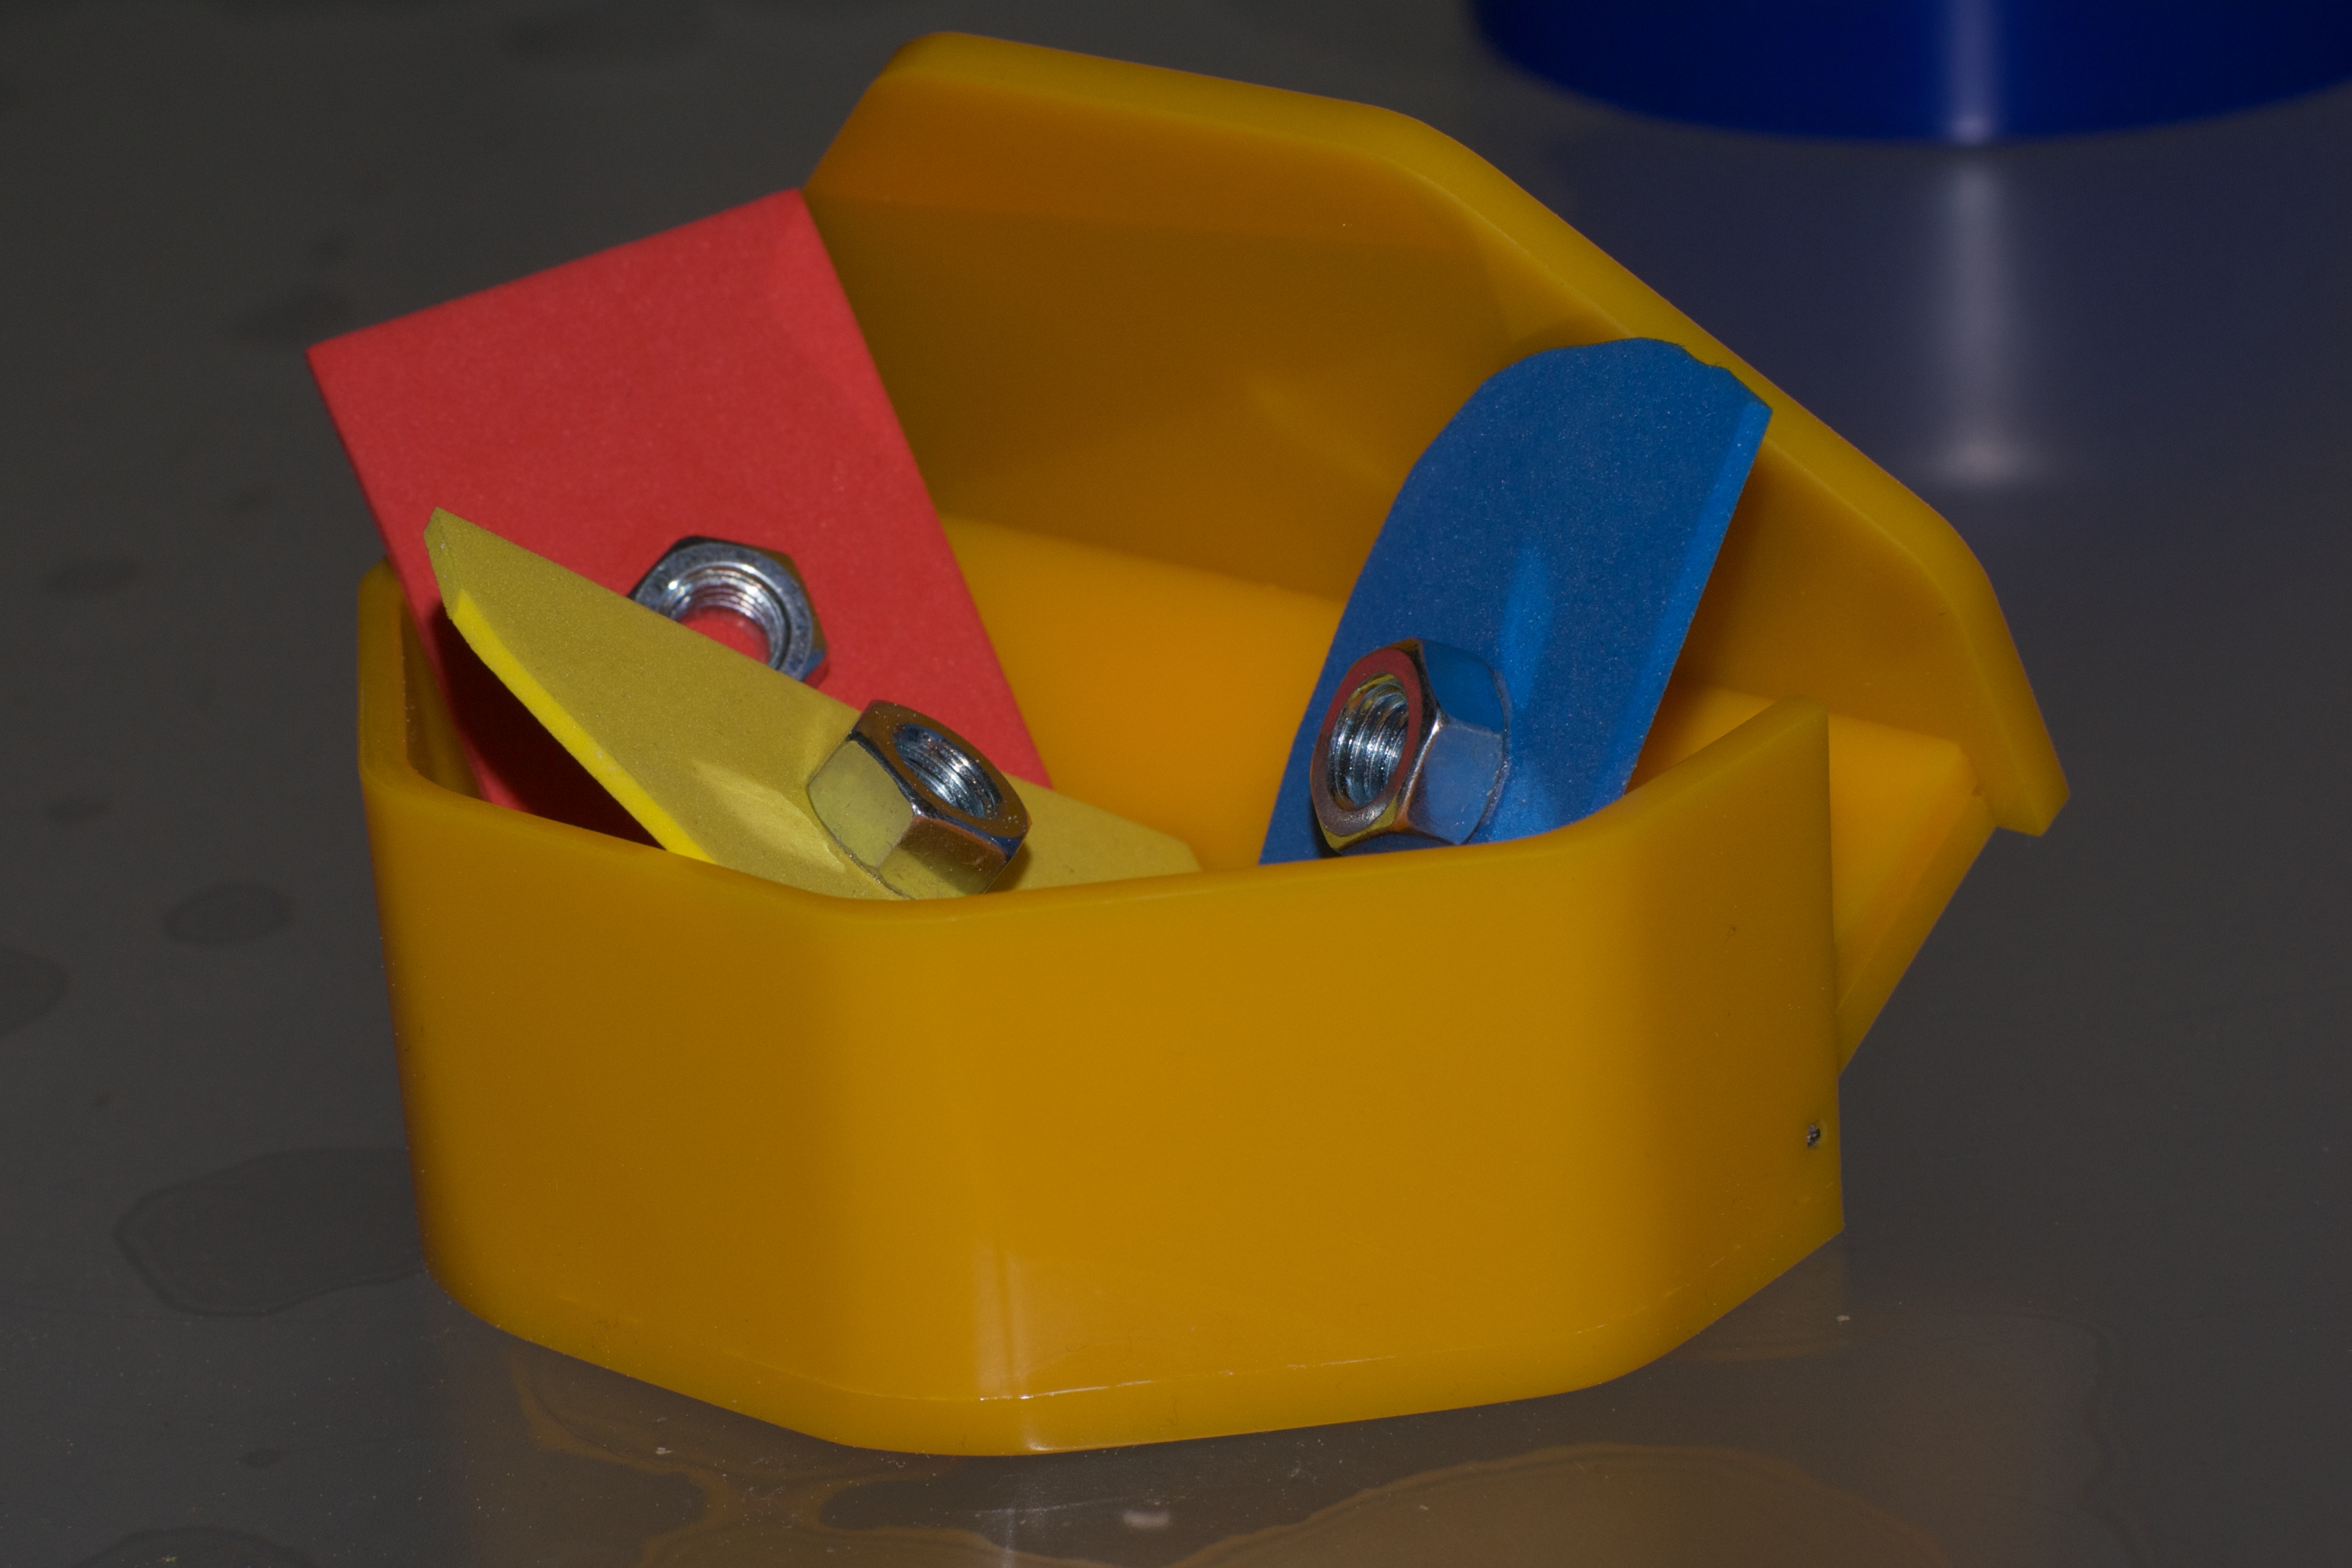
\includegraphics[height=2in]{img/SystemNeu/Container3EinbettungenTisch.jpg}
		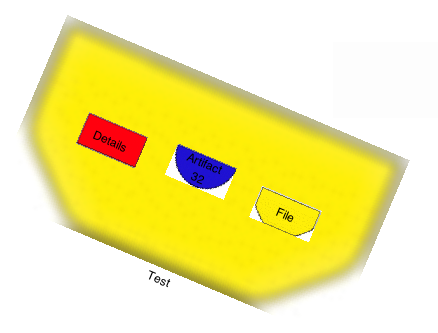
\includegraphics[height=2in]{img/SystemNeu/Container3EinbettungenScreen.png}
	\caption[Darstellung von Containern und eingebetteten Elementen]{\centering Darstellung von Containern und eingebetteten Elementen \par \centering (links Tischoberfläche, rechts Bildschirm)}
	\label{fig:img_SystemNeu_Container}
\end{figure}

Jene Information, die an die eingebetteten Elemente gebunden ist, wird auf beiden Kanälen nicht ohne explizite Benutzerinteraktion dargestellt. Fordern die Benutzer auf einem Eingabekanal die Darstellung der eingebetteten Information an, so wird diese auf dem sekundären, nicht kohärenten Ausgabekanal dargestellt. Eine Darstellung der angebundenen Information auf der Tischoberfläche würde durch die physisch vorhanden Modellelemente gestört. Die eingebetteten Submodelle bzw. die sonstigen digitalen Ressourcen werden also auf dem Bildschirm dargestellt, wobei Submodelle den aktuellen Modellzustand temporär ersetzen und andere Ressourcen mittels der im Betriebssystem definierten Standardapplikation geöffnet werden. 
% subsection ausgabe_von_information_zum_modell (end)

\subsection{Ausgabe zur Kontrolle des Systems} % (fold)
\label{sub:ausgabe_zur_kontrolle_des_systems}

Neben der eigentlichen Modellinformation wird auch Information ausgegeben, die zum Feedback über den Systemzustand oder der Kontrolle desselben notwendig ist. Wo möglich wird auch in diesem Fall die Tischoberfläche als primärer Ausgabekanal genutzt.

\subsubsection{Zustands- und Ereignismeldungen} % (fold)
\label{ssub:zustands_und_ereignismeldungen}

Bei der Verwendung der die Modellierung unterstützenden Werkzeuge muss den Benutzern Feedback über deren Erkennung bzw. den durch diese ausgelösten Änderung des Systemzustandes gegeben werden. Dabei ist zwischen jenen Interaktionen zu unterscheiden, die ein Ereignis auslösen und jenen, die den Systemzustand permanent ändern. Dieser Unterschied muss auch in der Visualisierung den Benutzern kommuniziert werden. Dabei kann es duch die vom System nicht beeinflussbaren physischen Werkzeugtokens zu potentiellen Mißverständnissen kommen. Wird ein Werkzeugtoken, das lediglich ein Ereignis auslöst (wie zum Beispiel das Markierungstoken), von den Modellierenden auf der Oberfläche belassen, kann dieses als unter Umständen als zustandsverändernd und nicht als ereignisauslösend wahrgenommen werden. 

\paragraph{Elementauswahl}

Wird mittels dem Markierungstoken ein Element ausgewählt, so müssen die Benutzer über die Erkennung der Markierung benachrichtigt werden. Dabei muss erkenntlich sein, welches Element ausgewählt wurde und wie lange die Auswahl gültig ist. Die Auswahl eines Elements ist grundsätzlich ein Ereignis, ist jedoch immer Teil einer umfassenderen Interaktion, in der die Benutzer das ausgewählte Element verwenden (z.B. dieses benennen). Deswegen wirkt das Markierungsereignis einige Sekunden nach, um den Benutzern die Gelegenheit zur Fortsetzung des Interaktionsablaufs zu geben. Eine permanente Markierung eines ausgewählten Elements ist insofern nicht wünschenswert, als dass etwaige fehlerhafte Markierungen (durch Fehlauswahl oder Fehlerkennung) dann zusätzlicher Benutzerinteraktion zur Korrektur bedürften. Deswegen werden Markierungen als Ereignisse mit längerer Wirkungsdauer interpretiert.

\begin{figure}[htbp]
	\centering
		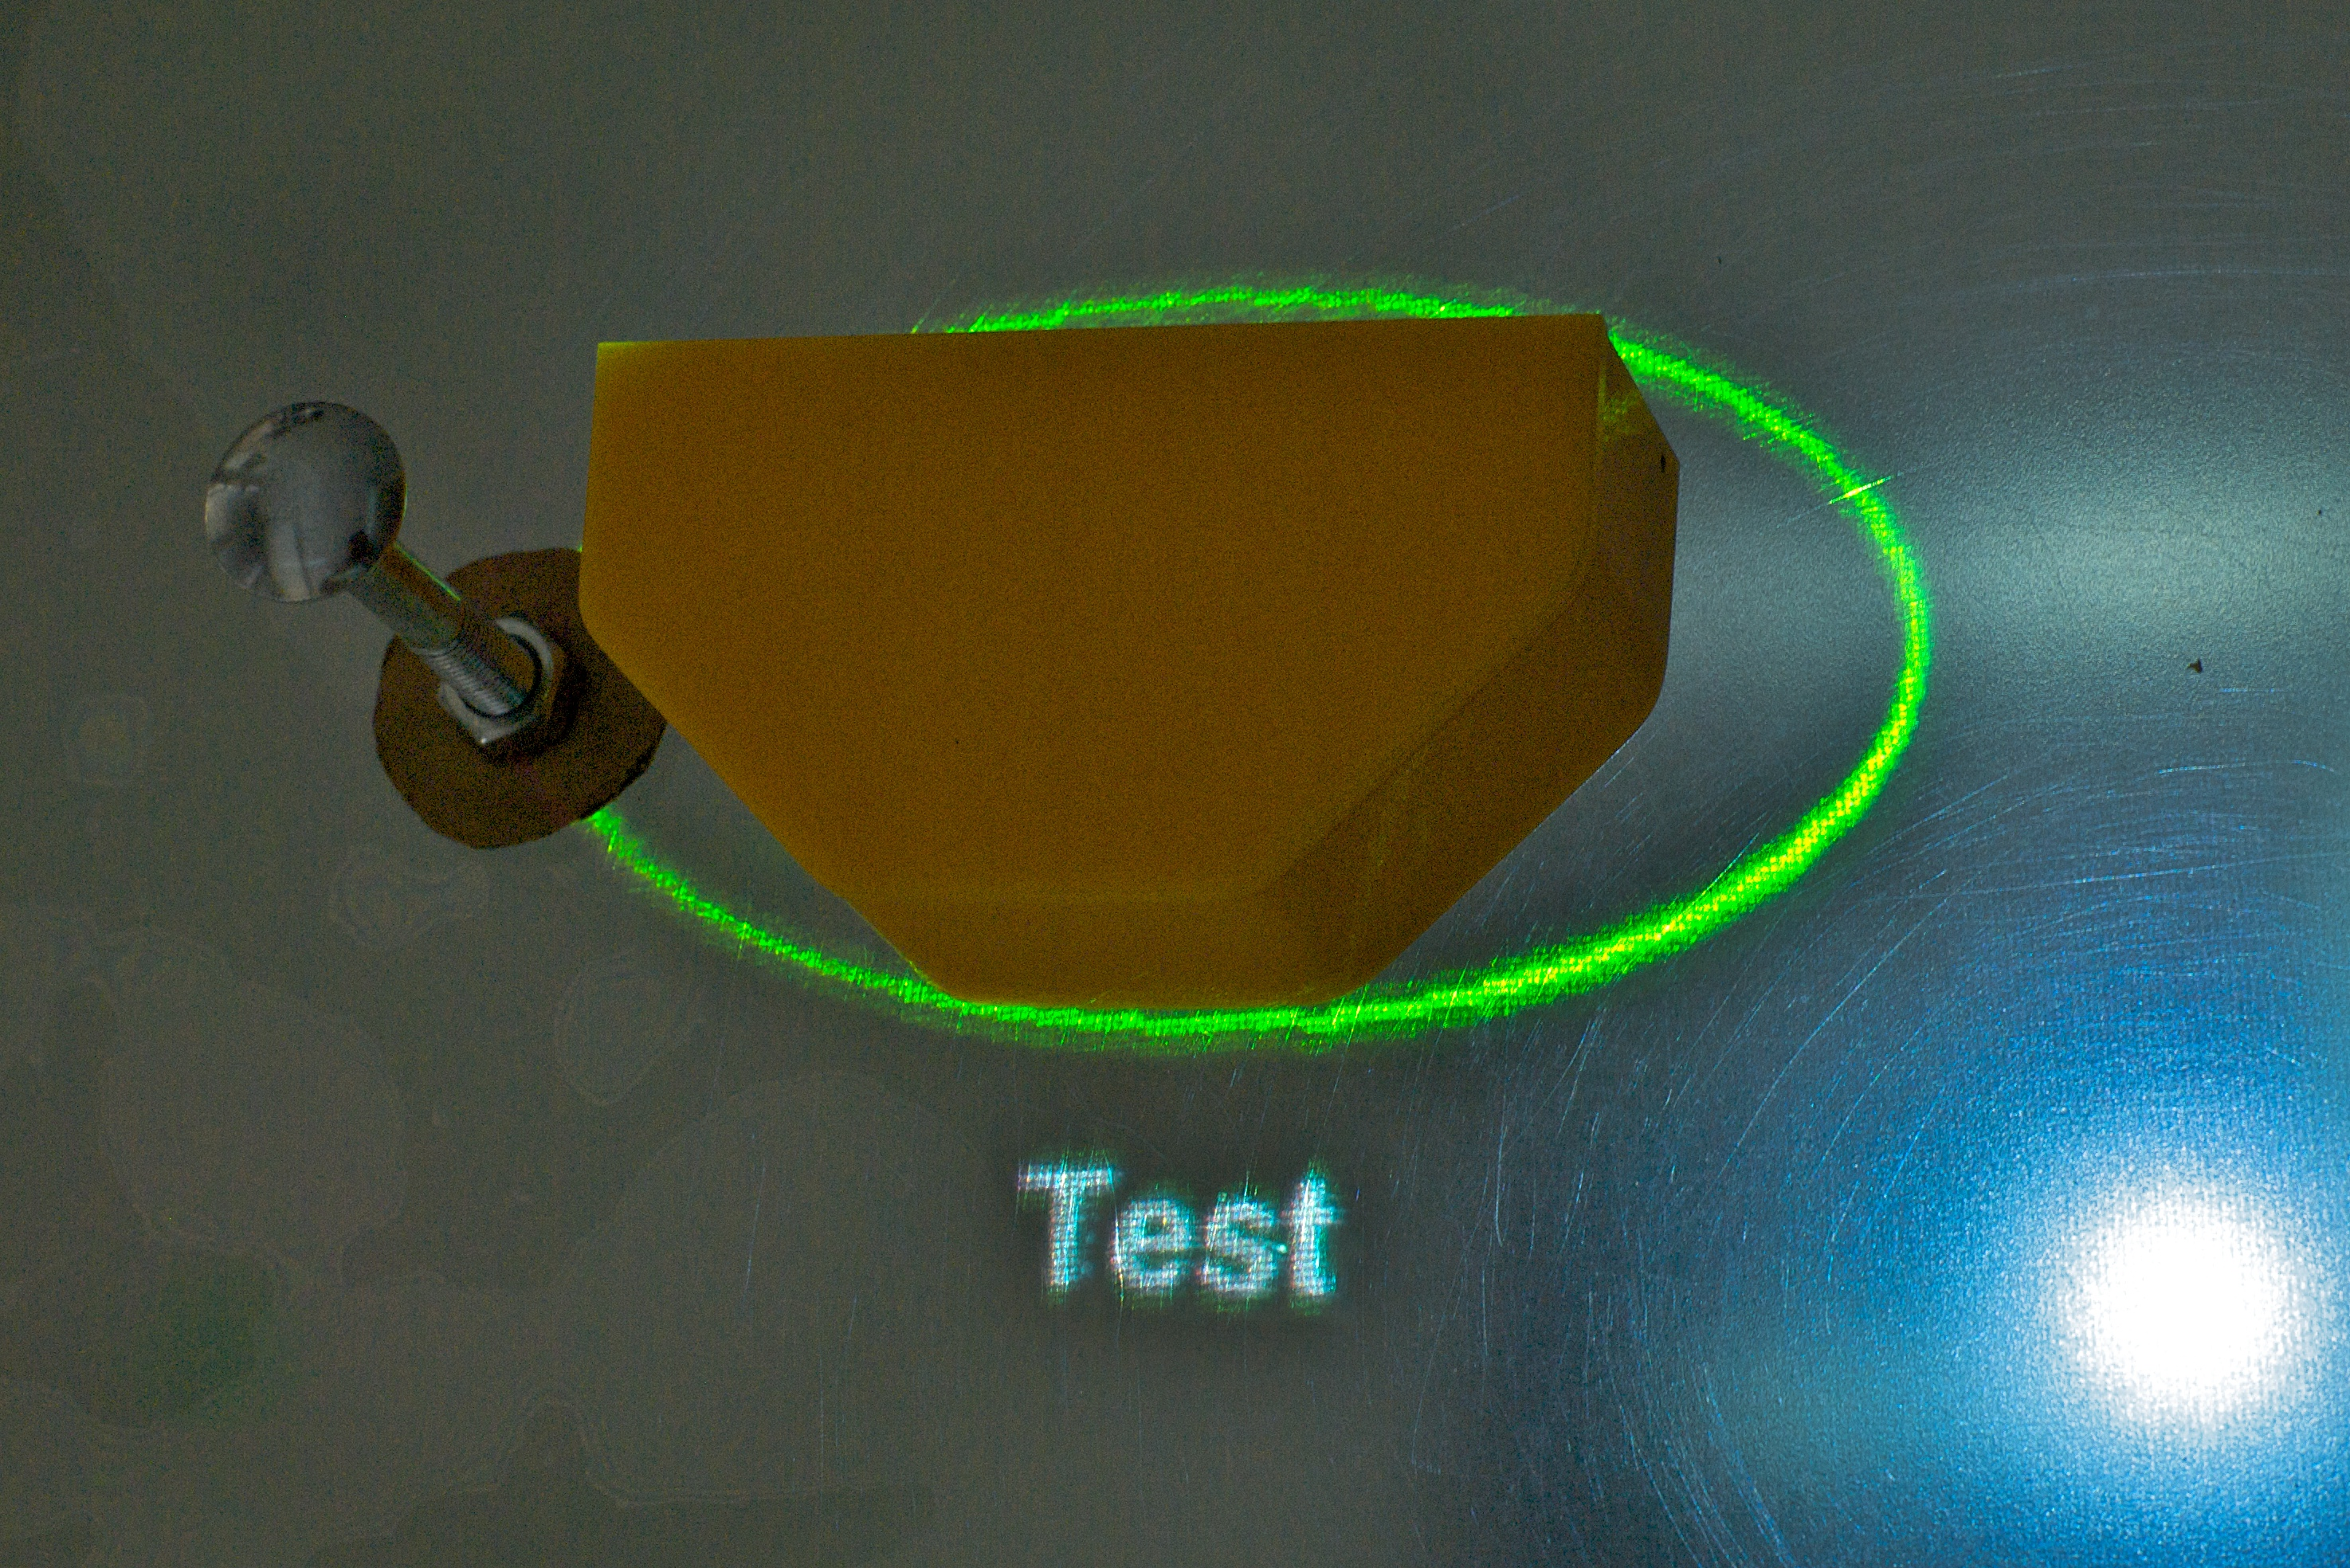
\includegraphics[height=2in]{img/SystemNeu/MarkierungTisch.jpg}
	\caption{Markierung von Modellelementen}
	\label{fig:img_SystemNeu_MarkierungTisch}
\end{figure}

Die Anzeige der Auswahl erfolgt auf beiden Ausgabekanälen mittels einer ovalen Markierung, die das ausgewählte Element umschließt (siehe Abbildung \ref{fig:img_SystemNeu_MarkierungTisch}). Diese wird solange angezeigt, bis die Interaktion, der sie zuzuordnen ist, abgeschlossen ist oder die Gültigkeitsdauer abgelaufen ist. Danach verschwindet sie selbständig ohne weiter Benutzerinteraktion.

\paragraph{Verbindungsherstellung}

Die Herstellung von Verbindungen kann auf zwei unterschiedliche Arten durch die Benutzer ausgelöst werden. Wird eine Verbindung duch die Auswahl zweier Modellelemente hergestellt, werden die eben beschriebenen ovalen Markierungen zur Visualisierung der Auswahl verwendet. Dabei kann es zur Auswahl eines Elements als Endpunkt einer gerichteten Verbindung kommen. Die ovale Markierung wechselt in diesem Fall die Farbe, um die erfolgreiche Erkennung einer Pfeilspitze rückzumelden. Nachdem beide Endpunkte erkannt und markiert wurden, wird unmittelbar die Verbindung hergestellt. Diese wird initial als einee Linie dargestellt, die in Farbe und Strichstärke hervorsticht, und in der Folge in einer Animation durch eine herkömmliche Verbindung ersetzt. Diese Animation dient dazu, das Ereignis der Verbindungsherstellung klar zu visualisieren und die Aufmerksamkeit der Benutzer auf dieses Ereignis zu lenken.

Werden zwei Elemente durch ihre räumliche Nähe zueinander in Beziehung gesetzt und eine Verbindung hergestellt, entfallen die ovalen Markierungen (da keine explizite Auswahl der Elemente erfolgt). Es wird lediglich die Animation zur Verbindungsherstellung dargestellt. Auf diesem Wege ist keine Herstellung von gerichteten Verbindern möglich. 

\paragraph{explizite Snapshots}

Im Zusammenhang mit der Speicherung der Modellierungshistorie (also der über die Zeit veränderten Modellzustände) ist es möglich, neben der automatischen Speicherung auch explizit der Aufnahme eines Snapshots auszulösen. Während bei der automatischen Speicherung kein Feedback an die Benutzer gegeben wird (da auch keine Interaktion zum Auslösen derselben stattfindet), wird im Falle einer expliziten Speicherung den Benutzern die erfolgreiche Durchführung der Aktion rückgemeldet. Die Speicherung des Snapshots ist ein Ereignis ohne zeitliche Ausdehnung und wird dementsprechend visualisiert. Dies erfolgt in Form eines roten Blitzes, der sowohl über die Tischoberfläche als auch den Bildschirm ausgegeben wird. Die Verwendung der gespeicherten Modellzustände und deren Visualisierung wird in Abschnitt \ref{ssub:abruf_der_modellierungshistorie} im Detail behandelt.

\paragraph{Löschmodus}

Im Gegensatz den in den vorangegangenen Abschnitten behandelten Werkzeugen löst der Einsatz des Lösch-Tokens kein Ereignis aus sondern schaltet das System in einen anderen Zustand, solange es auf der Oberfläche vorhanden ist. Dies spiegelt sich auch in der Visualisierung wieder. Solange das Lösch-Token von der Kamera erfasst wird, wird auf beiden Ausgabekanälen der Hintergrund des Modells (also die gesamte Tischoberfläche bzw. der gesamte Bildschirm) in roter Farbe dargestellt, während im Vordergrund nach wie vor der aktuelle Modellzustand visualisiert wird. Dies entspricht den Interaktionsmöglichkeiten der Benutzer -- das Modell kann nach wie vor manipuliert werden, jene Interaktionen, die aber im Normalfall eine Verbindung herstellen, löschen diese in diesem Modus wieder. Wird das Lösch-Token entfernt, wechselt der Hintergrund wieder auf die Standard-Farbe, das System reagiert auf dei betroffenen Interaktionen wieder mit der Herstellung eines Verbinders.

% subsubsection zustandsmeldungen (end)

\subsubsection{Abruf der Modellierungshistorie} % (fold)
\label{ssub:abruf_der_modellierungshistorie}

Der Abruf der Modellierungshistorie wird mit dem runden Kontroll-Token ausgelöst und kontrolliert. Hinsichtlich der Darstellung ist die Modellierungshistorie die erste der hier beschriebenen Zustands- und Ereignismeldungen, bei der keine kohärente Darstellung möglich ist. Auf der Tischoberfläche befinden sich zum Zeitpunkt der Aktivierung des Historienmodus alle Tokens, die im Elemente im aktuellen Modellzustand repräsentieren. Da der Historienmodus als Referenz dient, in der die Entstehung des Models rekapituliert werden kann, die gespeicherten Modellzustände aber im Allgemeinen nicht den aktuellen Zustand ersetzen sollen, verbleiben diese Tokens auch auf der Oberfläche. Damit kann nach Deaktivierung des Historienmodus der Modellierungsvorgang unmittelbar fortgesetzt werden. Die auf der Oberfläche befindlichen Tokens stören aber die Darstellung gespeicherter Modellzustände, da sie Teile verdecken und keinen Bezug zum projizierten Modell haben.

Die Information des Historienmodus wird deshalb ausschließlich auf dem sekundären Ausgabekanal -- dem Bildschirm -- dargestellt (die Kontrolle verbleibt mit dem runden Kontroll-Token auf der Tischoberfläche). Die gespeicherten Modellzustände ersetzen dabei den aktuellen Modellzustand, der im Normalbetrieb synchron zur Tischoberfläche dargestellt wird. Ist das System so konfiguriert, das der sekundäre Ausgabekanal nicht synchron betrieben wird, so wird er bei Erkennung des Historienmodus aktiviert.

\begin{figure}[htbp]
	\centering
		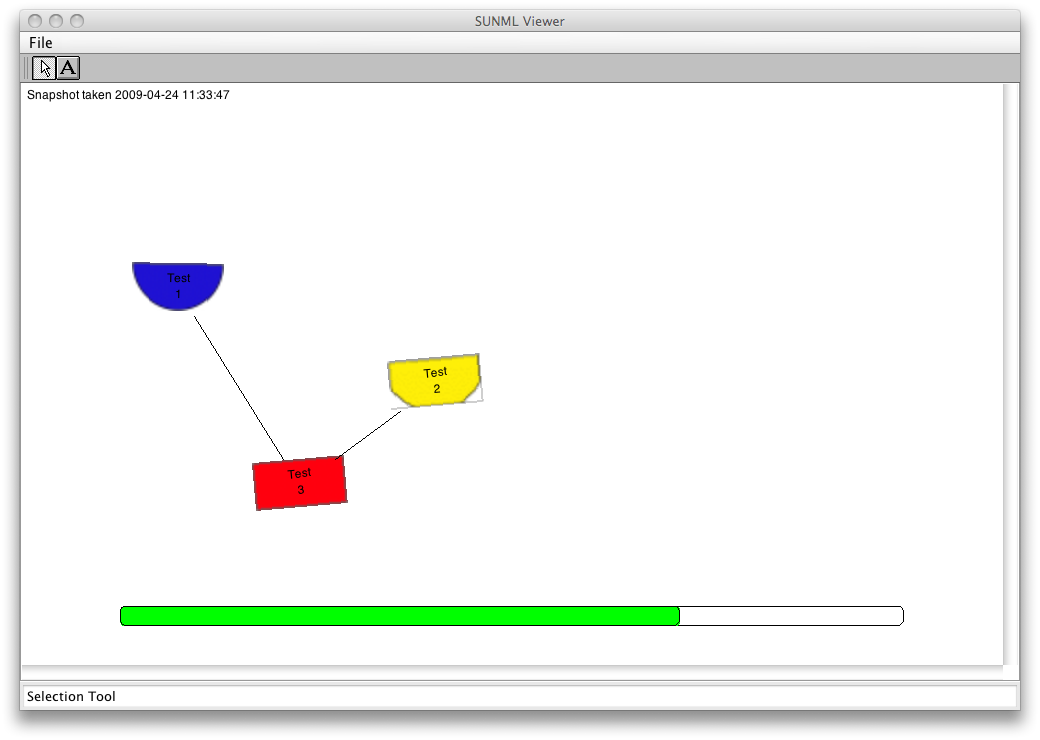
\includegraphics[height=2in]{img/SystemNeu/HistoryScreen.png}
	\caption{Darstellung der Modellierungshistorie}
	\label{fig:img_SystemNeu_HistoryScreen}
\end{figure}

Zusätzlich zur graphischen Darstellung des gespeicherten Modellzustandes wird ein Zeitstempel in der linken oberen Ecke eingeblendet, der den Zeitpunkt der Speicherung angibt. Am unteren Rand des Bildes wird ein Balken eingeblendet, der auf den relativen Zeitpunkt der Aufnahme (bezogen auf die Gesamtzahl der gespeicherten Zustände) angibt (siehe Abbildung \ref{fig:img_SystemNeu_HistoryScreen}). Die Schrittweite (also die Verlängerung des Balken, die durch das Umschalten auf einen unmittelbar folgenden Zustand verursacht wird) wird dazu dynamisch an die Anzahl der gespeicherten Modellzustände angepasst.

Ist der erste bzw. letzte Modellzustand erreicht, werden weitere entsprechende Kommandos durch Drehen des Kontroll-Tokens ignoriert. Die Benutzer werden durch einen vollständig leeren bzw. ausgefüllten Balken auf das Erreichen des jeweiligen Endpunktes hingewiesen. Wird das Kontroll-Token von der Tischoberfläche entfernt, so wird der Historienmodus deaktiviert. Die Darstellung auf dem sekundären Ausgabekanal wird wieder auf die synchrone Darstellung des aktuellen Modellzustandes geschalten bzw. wird diese deaktiviert, falls das System dementsprechend konfiguriert ist.

% subsubsection abruf_der_modellierungshistorie (end)
\subsubsection{Wiederherstellungsunterstützung} % (fold)
\label{ssub:wiederherstellungsunterstützung}

Im Rahmen des Abrufs der Modellierungshistorie kann von den Benutzern die Wiederherstellungsunterstützung aktiviert werden. Im Rahmen der Wiederherstellungsunterstützung leitet das System die Benutzer bei der Rekonstruktion eines gespeicherten Modellzustandes an. Dazu werden auf der Tischoberfläche und am Bildschirm (sofern aktiviert) -- also auf beiden Ausgabekanälen -- Hinweise angezeigt, wie der aktuelle Modellzustand verändert werden muss, um den gespeicherten Zustand wieder herzustellen. Da der aktuelle Modellzustand als Ausgangspunkt dient, kann eine kohärente Visualisierung zum Einsatz kommen.

Bei der Aktivierung der Wiederherstellungsunterstützung werden die im Modell befindlichen Verbinder ausgeblendet, da diese nicht manuell verändert werden müssen. Die notwendige manuelle Intervention der Benutzer zur Wiederherstellung beschränkt sich auf die Platzierung der Modellierungstokens an die dem gespeicherten Modellzustand entsprechenden Orte. In der ersten Phase werden vom System schrittweise alle Tokens markiert, die im aktuellen Modell enthalten sind und im gespeicherten Modellzustand nicht vorhanden sind -- also entfernt werden müssen. Schrittweise heißt in diesem Zusammenhang, dass immer nur ein Token markiert wird, sobald dieses entfernt wurde, wird das nächste Token zur Entfernung markiert. Die Markierung ist als rote, ovale Hinterlegung des Tokens umgesetzt.

In der zweiten Phase werden jene Tokens behandelt, die sowohl im aktuellen als auch im gespeicherten Modellzustand enthalten sind, sich aber jeweils an unterschiedlichen Positionen befinden -- also verschoben werden müssen. Dazu wird wiederum schrittweise eine Markierung an der Zielposition des Tokens eingeblendet und diese mit einem Pfeil mit der aktuellen Position des betroffenen Tokens verbunden (siehe Abbildung \ref{fig:img_SystemNeu_WiederherstellungTisch}).

In der letzten Phase werden alle Tokens hinzugefügt, die im aktuellen Modell nicht vorhanden sind, es im gespeicherten Modellzustand aber waren. Diese werden schrittweise durch grüne, ovale Markierungen an den jeweiligen Positionen angezeigt, wobei die Benennung des Tokens in die Markierung eingeblendet wird, um das jeweilige zu platzierende Element identifizieren zu können.

\begin{figure}[htbp]
	\centering
		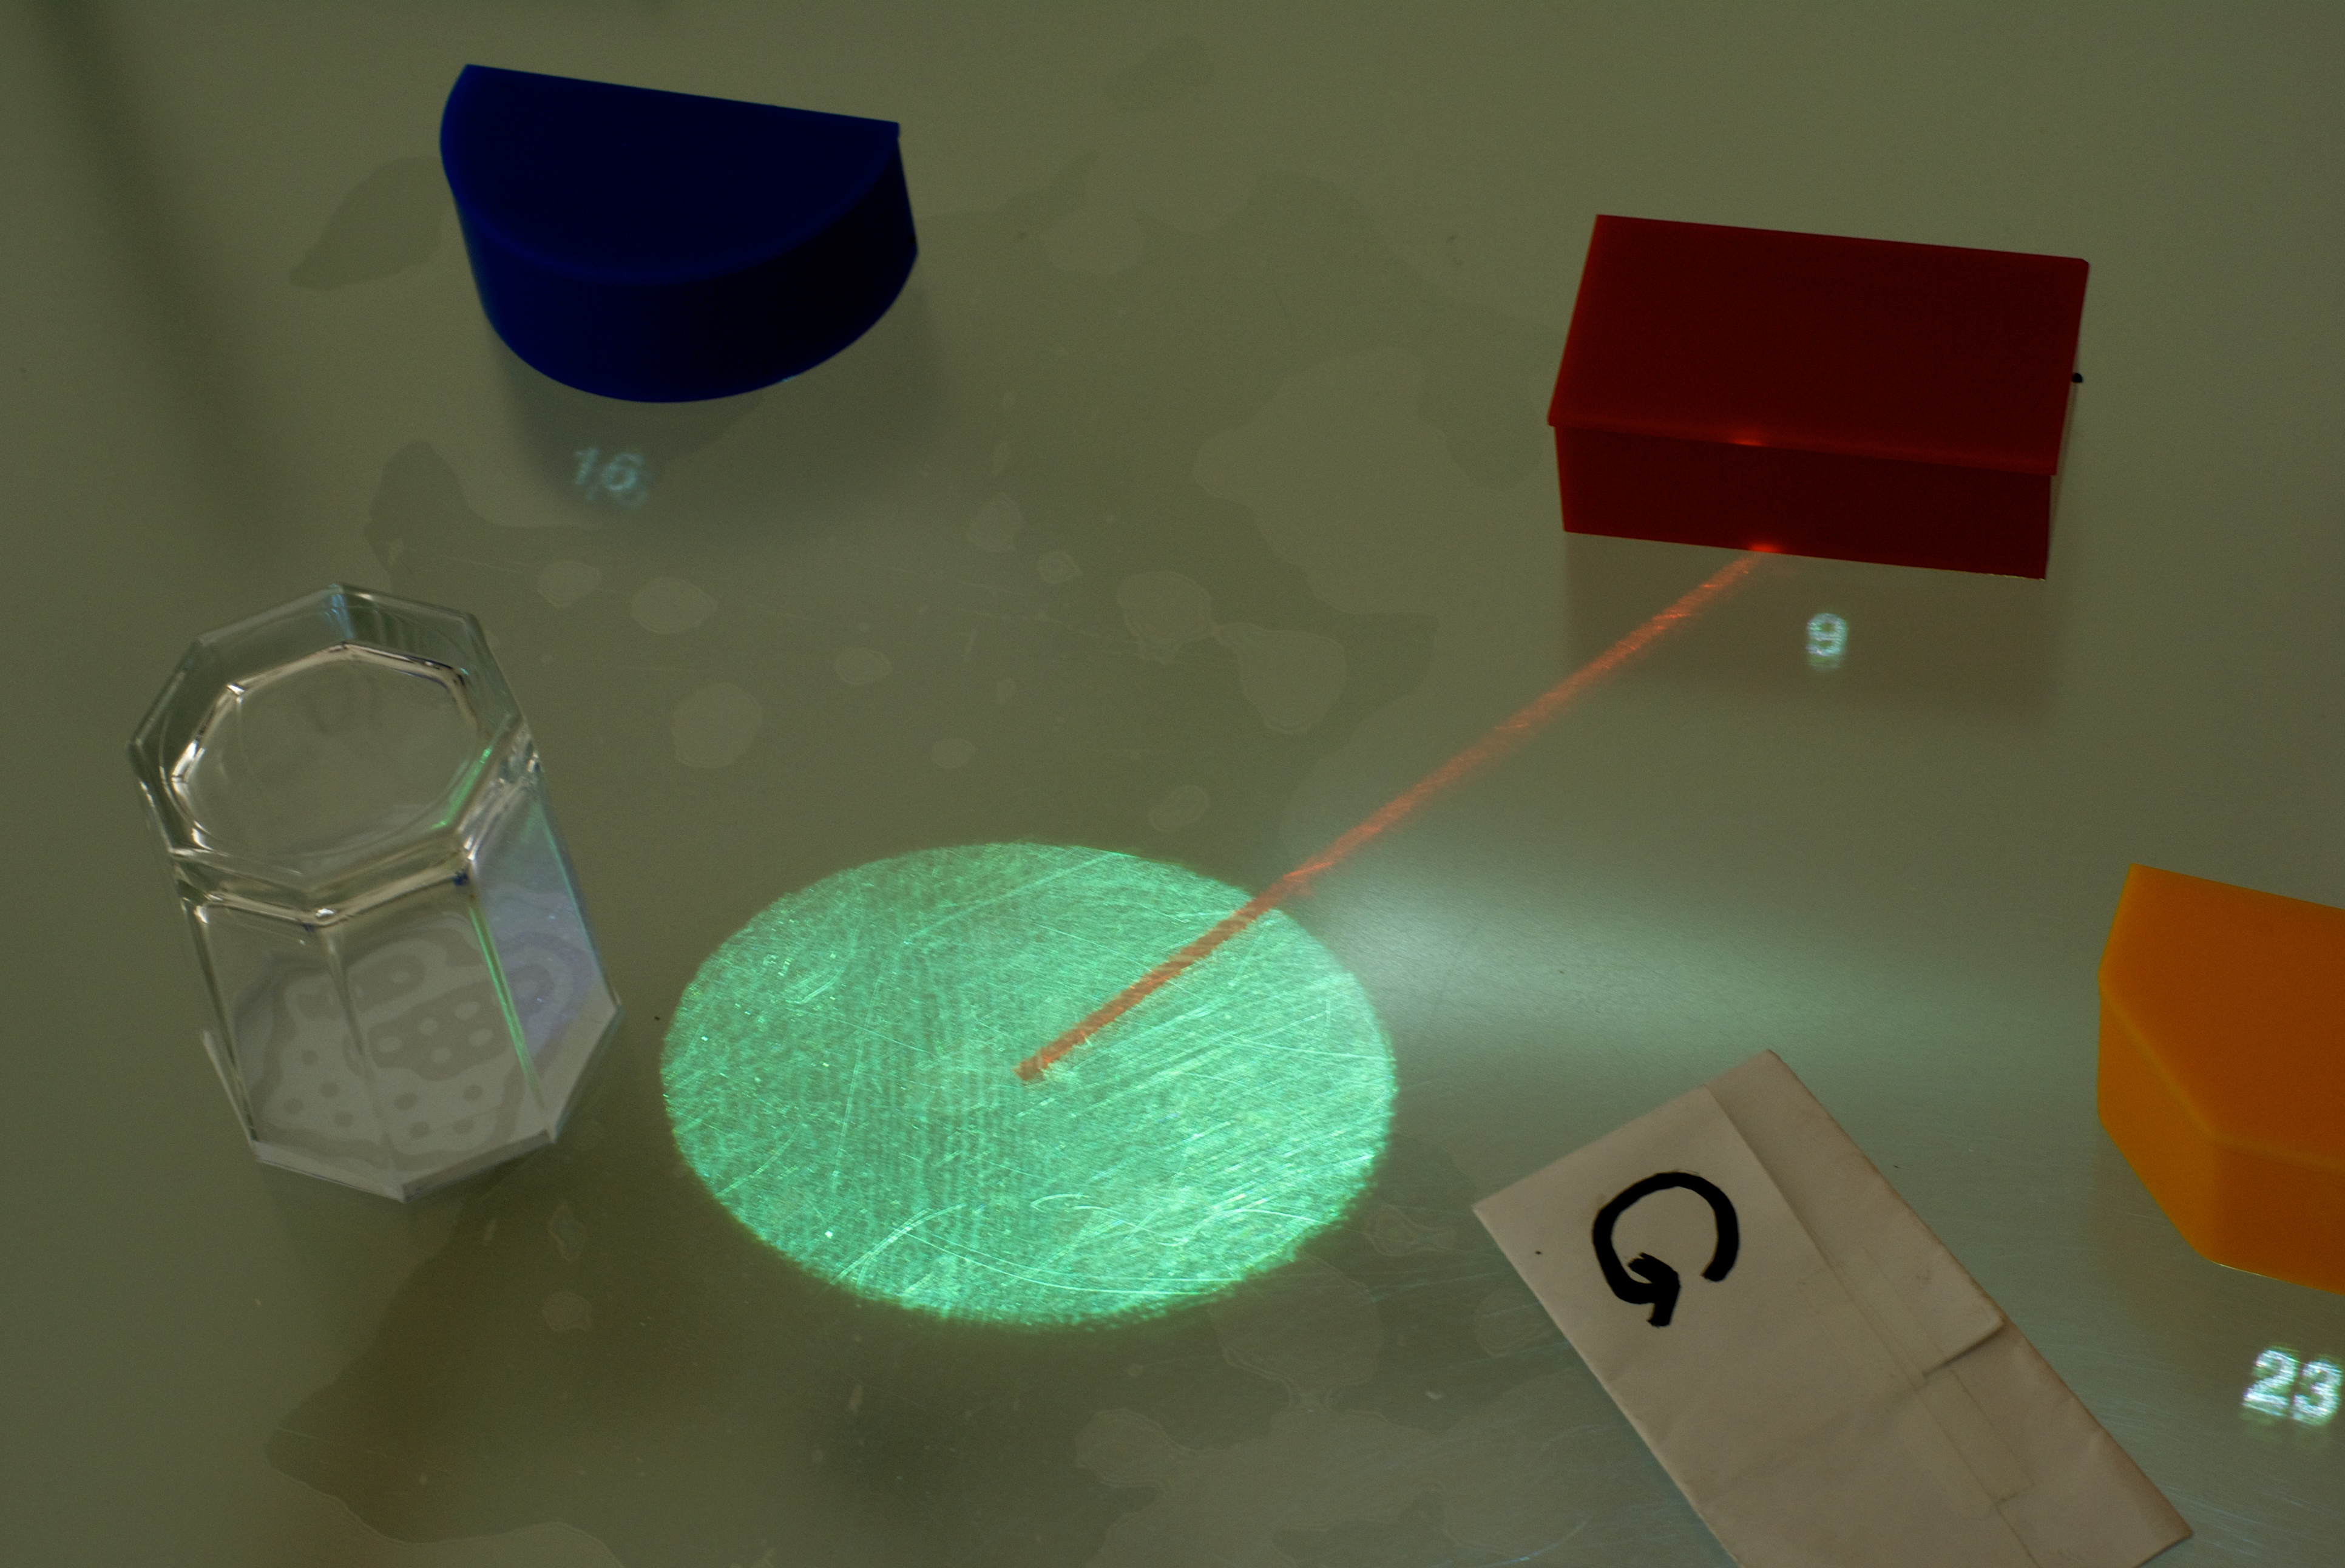
\includegraphics[height=2in]{img/SystemNeu/WiederherstellungTisch.jpg}
	\caption{Unterstützung der Wiederherstellung von Modellzuständen}
	\label{fig:img_SystemNeu_WiederherstellungTisch}
\end{figure}

Die zur Rekonstruktions des Modellzustandes notwendigen Schritte sind nicht vorberechnet sondern werden vielmehr Schritt für Schritt aus der aktuell auf der Tischoberfläche befindlichen Token-Konstellation extrahiert. Dadurch ist es möglich, auch irrtümlicherweise während der Wiederherstellung entfernte, hinzugefügte oder vor allem verschobene Tokens zu korrigieren, auch wenn die Rekonstruktion grundsätzlich schon in eine spätere Phase getreten wäre. So würde das System beispielsweise nach Abschluss eines Schrittes in der dritten Phase (Elemente hinzufügen) auf eine Anweisung in der zweiten Phase (Verschieben) zurückgreifen, wenn durch das Hinzufügen ein anderes, bereits an der korrekten Position befindliches Element verschoben worden wäre.

Sobald sich die Positionen der Tokens mit jenen des gespeicherten Modellzustandes decken, ist die notwendige Benutzerintervention zur Wiederherstellung abgeschlossen. Die Benutzer werden nun ggf. aufgefordert, das Historien-Kontroll-Token und das Wiederherstellungs-Token zu entfernen (sofern sich diese noch auf der Oberfläche befinden). Dieser Schritt schließt die Wiederherstellungsunterstützung ab. Das System blendet die Verbinder (nun aus dem gespeicherten Modellzustand) wieder ein und zeigt damit den (neuen) aktuellen Modellzustand an. 

% subsubsection wiederherstellungsunterstützung (end)
% subsection ausgabe_zur_kontrolle_des_systems (end)

% section ausgabe_von_information (end)

\section{Umsetzung der Ausgabe mit Software} % (fold)
\label{sec:umsetzung_der_ausgabe_mit_software}

\subsection{Ausgabe des Modellzustands} % (fold)
\label{sub:einsatz_von_jhotdraw}

Bildschirm und Projektor

\subsubsection{Kalibrierung der Ausgabe} % (fold)
\label{ssub:kalibrierung_der_ausgabe}

Der Projektor, der die Information auf die Tischoberfläche projiziert, ist aus Gründen der Transportierbarkeit nicht fix im Boden des Tisches eingebaut. Deswegen ist nach dem Aufbau der Systems im Allgemeinen die projizierte Version des Modells nicht deckungsgleich mit der Position der physischen Tokens. Es kann eine Verschiebung entlang beider Achsen auftreten, die alle zu den physischen Tokens ausgegebene Information von diesen absetzt. Dadurch kann die Information unter Umständen nicht mehr eindeutig zugeordnet werden.

Aus diesem Grund ist die Position der projizierten Modellversion einstellbar, die Kalibrierung muss einmalig nach dem Aufbau des Werkzeugs vorgenommen werden. Aufgrund der Verwendung des Umlenkspiegels kann es nicht nur zu einer Verschiebung der Information auf der X- oder Y-Achse kommen, es können auch Spreizungen oder Stauchungen auftreten, welche den Projektions-Fehler von links nach rechts bzw. von oben nach unten zunehmen lassen. Auch diese Spreizungen oder Stauchungen sind softwareseitig im Rahmen der Kalibrierung korrigierbar. 

% subsubsection kalibrierung_der_ausgabe (end)

\subsection{Weitere Ausgabekanäle} % (fold)
\label{sub:weitere_ausgabekanäle}

Verteilter Viewer

% subsection weitere_ausgabekanäle (end)
% section umsetzung_der_ausgabe_mit_software (end)

% chapter visualisierung (end)